%%%%%%%%%%%%%%%%%%%%%%%%%%%%%%%%%%%%%%%%%%%%%%%%%%%%%%%%%%%%%%%%%%%%%%%%%%%%%%%%
% Sweave/Knitr init


%%%%%%%%%%%%%%%%%%%%%%%%%%%%%%%%%%%%%%%%%%%%%%%%%%%%%%%%%%%%%%%%%%%%%%%%%%%%%%%%

\documentclass{article}\usepackage{graphicx, color}
%% maxwidth is the original width if it is less than linewidth
%% otherwise use linewidth (to make sure the graphics do not exceed the margin)
\makeatletter
\def\maxwidth{ %
  \ifdim\Gin@nat@width>\linewidth
    \linewidth
  \else
    \Gin@nat@width
  \fi
}
\makeatother

\IfFileExists{upquote.sty}{\usepackage{upquote}}{}
\definecolor{fgcolor}{rgb}{0.2, 0.2, 0.2}
\newcommand{\hlnumber}[1]{\textcolor[rgb]{0,0,0}{#1}}%
\newcommand{\hlfunctioncall}[1]{\textcolor[rgb]{0.501960784313725,0,0.329411764705882}{\textbf{#1}}}%
\newcommand{\hlstring}[1]{\textcolor[rgb]{0.6,0.6,1}{#1}}%
\newcommand{\hlkeyword}[1]{\textcolor[rgb]{0,0,0}{\textbf{#1}}}%
\newcommand{\hlargument}[1]{\textcolor[rgb]{0.690196078431373,0.250980392156863,0.0196078431372549}{#1}}%
\newcommand{\hlcomment}[1]{\textcolor[rgb]{0.180392156862745,0.6,0.341176470588235}{#1}}%
\newcommand{\hlroxygencomment}[1]{\textcolor[rgb]{0.43921568627451,0.47843137254902,0.701960784313725}{#1}}%
\newcommand{\hlformalargs}[1]{\textcolor[rgb]{0.690196078431373,0.250980392156863,0.0196078431372549}{#1}}%
\newcommand{\hleqformalargs}[1]{\textcolor[rgb]{0.690196078431373,0.250980392156863,0.0196078431372549}{#1}}%
\newcommand{\hlassignement}[1]{\textcolor[rgb]{0,0,0}{\textbf{#1}}}%
\newcommand{\hlpackage}[1]{\textcolor[rgb]{0.588235294117647,0.709803921568627,0.145098039215686}{#1}}%
\newcommand{\hlslot}[1]{\textit{#1}}%
\newcommand{\hlsymbol}[1]{\textcolor[rgb]{0,0,0}{#1}}%
\newcommand{\hlprompt}[1]{\textcolor[rgb]{0.2,0.2,0.2}{#1}}%

\usepackage{framed}
\makeatletter
\newenvironment{kframe}{%
 \def\at@end@of@kframe{}%
 \ifinner\ifhmode%
  \def\at@end@of@kframe{\end{minipage}}%
  \begin{minipage}{\columnwidth}%
 \fi\fi%
 \def\FrameCommand##1{\hskip\@totalleftmargin \hskip-\fboxsep
 \colorbox{shadecolor}{##1}\hskip-\fboxsep
     % There is no \\@totalrightmargin, so:
     \hskip-\linewidth \hskip-\@totalleftmargin \hskip\columnwidth}%
 \MakeFramed {\advance\hsize-\width
   \@totalleftmargin\z@ \linewidth\hsize
   \@setminipage}}%
 {\par\unskip\endMakeFramed%
 \at@end@of@kframe}
\makeatother

\definecolor{shadecolor}{rgb}{.97, .97, .97}
\definecolor{messagecolor}{rgb}{0, 0, 0}
\definecolor{warningcolor}{rgb}{1, 0, 1}
\definecolor{errorcolor}{rgb}{1, 0, 0}
\newenvironment{knitrout}{}{} % an empty environment to be redefined in TeX

\usepackage{alltt}
\usepackage[margin=1in]{geometry}
\usepackage{algorithm, color, algpseudocode, amsmath, url, geometry, ctable}
\usepackage{titlesec, siunitx}
\usepackage[round,authoryear]{natbib}
\usepackage[section]{placeins}  % keep floats in their place.
\usepackage{authblk}            % Listing Author affiliations
\usepackage[hypcap]{caption}


%draft mode
\usepackage[colorinlistoftodos, textwidth=4cm, shadow]{todonotes}
\usepackage[displaymath, tightpage]{preview}
\setlength{\marginparwidth}{1.2in}

% styling
\newcommand{\subsubsubsection}[1]{\paragraph{#1}}
\renewcommand\Affilfont{\itshape\small}  %authblk

% shortcuts 
\newcommand{\mb}{MAGeT-Brain }
\newcommand{\ants}{ANTS }
\newcommand{\animal}{ANIMAL }
\newcommand{\adnidataset}{ADNI1:Complete 1Yr 1.5T }
\newcommand{\FEPdataset}{SZ-FEP }

% title and authors
\title{Bootstrapping Multi-atlas Hippocampal Segmentation with \mb}
\author[1]{Jon Pipitone}
\author[1]{Matt T. Park}
\author[1]{Julie Winterburn}
\author[1]{Tristram A. Lett}
\author[2,3]{Jason P. Lerch}
\author[4]{Jens C. Pruessner}
\author[4]{Martin Lepage}
\author[1,5]{Aristotle Voineskos}
\author[1,5,6]{M. Mallar Chakravarty}
\author[ ]{Alzheimer's Disease Neuroimaging Initiative}
\affil[1]{Kimel Family Translational Imaging-Genetics Lab, Centre for Addiction and
Mental Health, Toronto, ON, Canada}
\affil[2]{Neurosciences and Mental Health, Hospital for Sick Children, Toronto,
ON,Canada}
\affil[3]{Department of Medical Biophysics, University of Toronto, Toronto, ON,
Canada}
\affil[4]{Brain Imaging Group, Douglas Hospital Research Centre, Verdun, QC, Canada}
\affil[5]{Department of Psychiatry, University of Toronto, Toronto, ON, Canada}
\affil[6]{Institute of Biomedical Engineering, University of Toronto, Toronto,
ON, Canada}

\renewcommand\Authands{ and }

\date{}

\begin{document}
\maketitle

\begin{abstract}
\end{abstract}

\parbox{4in}{
\textbf{Contact:} \\
Jon Pipitone and M. Mallar Chakravarty \\
Kimel Family Translation Imaging-Genetics Research Laboratory \\
Research Imaging Centre \\
Centre for Addiction and Mental Health \\
250 College St. \\
Toronto, Canada   M5T 1R8 \\
jon.pipitone@camh.ca; mallar.chakravarty@camh.ca}


%%%%%%%%%%%%%%%%%%%%%%%%%%%%%%%%%%%%%%%%%%%%%%%%%%%%%%%%%%%%%%%%%%%%%%%%%%%%%%%%
%                               INTRODUCTION
%%%%%%%%%%%%%%%%%%%%%%%%%%%%%%%%%%%%%%%%%%%%%%%%%%%%%%%%%%%%%%%%%%%%%%%%%%%%%%%%
\section{Introduction}

The hippocampus is a brain structure situated in the medial temporal
lobe, and has long been associated with learning and memory
\citep{DenHeijer2012,Scoville2000}.  The hippocampus is of interest to neuroscientists because it is implicated in
many forms of brain disfunction, including Alzheimer's disease
\citep{Sabuncu2011} and schizophrenia \citep{Narr2004,Karnik-Henry2012}.  In
neuroimaging studies, structural magnetic resonance images (MRI) are often used for the volumetric assessment of the hippocampus.  As such, accurate segmentation of the
hippocampus and its subregions in MRI is a necessary first step to better
understand interindividual variability of neuroanatomy of subjects. Typically, the gold standard for
neuroanatomical segmentation is manual delineation by an expert human rater. However,
the rapid increase in the number of available MRI data and the time and expertise
required for manual segmentation makes this increasingly difficult
\citep{Mazziotta1995,Mazziotta2001,Mazziotta,Pausova2007}.
Further, there is significant variation between segmentation protocols regarding
specific anatomical boundaries of the hippocampus \citep{Geuze2004} and this has
led to efforts to create an unified hippocampal segmentation protocol
\citep{Jack2011}.  

Automated segmentation techniques that are reliable, objective, and reproducible
can be considered complementary to manual segmentation.  In the case of classical
model-based segmentation methods \citep{Haller1997,Csernansky1998}, an MRI atlas
that was previously manually labelled by an expert rater is matched to target
images using nonlinear registration methods.  The resulting nonlinear
transformation is applied to the manual labels (i.e. {\em label propagation}) to
move them into the target image space.  While this methodology has been used
successfully in several contexts
\citep{Chakravarty2008,Chakravarty2009,Collins1995,Haller1997}, it is limited
in accuracy by the introduction of errors due inaccuracies in the nonlinear
transformation itself, partial volume effects in label resampling, and
irreconcilable differences between the neuroanatomy represented within the atlas
and target images.
 
One methodology that can be used to mitigate these sources of errors involves
the use of multiple manually segmented atlases and probabilistic segmentation
techniques, such as those found in the FreeSurfer package \citep{Fischl2002}.
FreeSurfer uses a probabilistic atlas of anatomical and tissue classes along
with spatial constraints for class labels encoded using a Markov random field
model to segment the entire brain.  

More recently, many groups have been using multiple atlases to improve overall
segmentation accuracy (i.e. multi-atlas segmentation) over model-based approaches
\citep{Heckemann2006,Heckemann2011,Collins2010,Lotjonen2010,Aljabar2009,Leung2010,Wolz2010}.
Each atlas image is registered to a target image, and label propagation is
performed to produce several labellings of the target image (one from each
atlas). A {\it label fusion} technique, such as voxel-wise voting, is used to
merge these labels into a definitive segmentation for the target.  In addition,
weighted voting procedures that use {\em atlas selection} techniques are often
used to exclude atlases from label fusion that are dissimilar to a target image
in order to reduce error from unrepresentative anatomy \citep{Aljabar2009}.
This involves the selection of a subset of atlases using a similarity metric
such a cross-correlation \citep{Aljabar2009} or normalized mutual information.
Such selection has the added benefit of significantly reducing the number of
nonlinear registrations.  For example \citet{Collins2010}
demonstrated that only 14 atlases, selected based on highest similarity between
medial temporal lobe neuroanatomy as evaluated by normalized mutual information
\citep{Studholme1999} from a library of 80 atlases, were required to achieve
accurate segmentations of the hippocampus.  Several methods have been explored
for label fusion including the STAPLE algorithm \citep{Warfield2004} that
computes a probabilistic segmentation using an expectation maximization
framework from an set of competing segmentations; or others where a subset of
segmentations can be estimated using metrics such as the sum of squared
differences in the regions of interest to be segmented \citep{Coupe2011}.

However, many of these methods require significant investment of time and
resources for the creation of the atlas library; ranging from atlas libraries
that require between 30 \citep{Heckemann2006} and 80 \citep{Collins2010}
manually segmented atlases.  This strategy has the main drawback of being
inflexible as it does not easily accommodate varying the definition of the
hippocampal anatomy (such as the commonly used heuristic of subdividing the
hippocampus in to head, body, and tail \citep{Poppenk2011,Pruessner2000}).
Furthermore, none of these methods have demonstrated sufficient flexibility to
accommodate atlases that are somehow exceptional such as those derived from
serial histological data \citep{Chakravarty2006,Yelnik2007} or high-resolution MRI
data that enables robust identification of hippocampal subfields
\citep{Winterburn2013,Yushkevich2009,Mueller2009,VanLeemput2009,Wisse2012}.  Due to
the recent availability of the latter, there has been increased interest in the
use of probabilistic methods for the identification of the hippocampal subfields
on standard T1-weighted images.  Our group recently demonstrated that through
use of an intermediary automated segmentation stage, robust and accurate
segmentation of the striatum, pallidum, and thalamus using a single atlas
derived from serial histological data is possible \citep{MallarChakravarty2012}.
The novelty of this manuscript is the extension our multi-atlas methodology to
the hippocampus using more than a single input atlas, while simultaneously
limiting the number of possible inputs used during segmentation, and
demonstrating that accurate identification of the hippocampal subfields is
indeed possible using this methodology.

There are few methods that have attempted to perform multi-atlas segmentation
with a limited number of input atlases. The LEAP algorithm is an elegant
modification to the basic multi-atlas strategy \citep{Wolz2010} in which the
atlas library is grown, beginning with a set of manually labelled atlases, and
successively incorporating unlabelled target images after themselves being
labelling using multi-atlas techniques. The sequence in which target images are
labelled is chosen so that the similarity between the atlas images and the
target images is minimised at each step, effectively allowing for deformations
between very dissimilar images to be broken up into sequences of smaller
deformations.  Although \citet{Wolz2010} begin with an atlas library of 30 MR
images, this method could theoretically work using a much smaller atlas library.
In their validation, LEAP was used to segment the whole hippocampus in the
ADNI-1 baseline dataset, achieving a mean Dice score of 0.85 with manual
segmentations.

To the best of our knowledge there are only two other segmentation methods that
attempt to define the hippocampal subfields using standard T1-weighted data.
The first is included with the FreeSurfer package \citep{VanLeemput2009}.  This
work is limited as it omits the tail of the hippocampus and the segmentation
protocol has yet to be fully validated.  Nonetheless, they demonstrate the
applicability of their work using data from 10 subjects.  In the second method,
\citet{Yushkevich2009} hippocampal subfields were acquired and labelled on
high-resolution MRI data from post-mortem medial temporal lobe samples. Using
nonlinear registration guided by manually derived hippocampus masks and specific
landmarks, the authors demonstrated accurate parcellation of hippocampal subfields in
unlabelled MRI volumes. 

Here we address the issue of limiting the number of input atlases by tuning our
algorithm, for segmentation of the entire hippocampus, using a multi-fold
experiment performed on a subset Alzheimer's Disease Neuroimaging Initiative
(ADNI) 1 dataset. Based on the parameters we find in our experiment, we validate
our algorithm using all of the data available in the ADNI Complete 1Yr sample
and compare our segmentations to the other segmentations that are available
through the ADNI informatics portal.  To ensure that we have not over-fit our
parameters to the aging or neurodegenerative brain, we also apply our
segmentations to a dataset of normal controls and individuals suffering from
first episode psychosis. Finally, we perform a leave-one-out validation
experiment to determine if the subfields can be accurately identified using our
multi-atlas framework. 


%%%%%%%%%%%%%%%%%%%%%%%%%%%%%%%%%%%%%%%%%%%%%%%%%%%%%%%%%%%%%%%%%%%%%%%%%%%%%%%%
%                               METHODS
%%%%%%%%%%%%%%%%%%%%%%%%%%%%%%%%%%%%%%%%%%%%%%%%%%%%%%%%%%%%%%%%%%%%%%%%%%%%%%%%
\section{Methods}

%%%%%                     MAGeT Brain Algorithm                            %%%%%

\subsection{The \mb Algorithm}
In this paper, we will use the term {\em label} to mean any segmentation (manual or 
derived) of an MR image.  {\em Label propagation}, or {\em labelling}, is the 
process by which two images are registered and the resulting transformation 
is applied to the labels from one image to bring them into alignment with the 
other image. We will use the term {\em atlas} to mean a manually segmented image,
and the term {\em template} to mean an automatically segmented image (i.e. 
via label propagation). The terms {\em atlas library} and {\em template library} 
describe any set of such images.Additionally, we will use the term {\em target} 
to refer to an unlabelled image that is undergoing segmentation.

The simplest form of multi-atlas segmentation, (which we will call {\em basic 
multi-atlas segmentation}), involves three steps.  First, each labelled 
input image (i.e. atlas or template) is registered to an unlabelled target image.
Second, the labels from each image are propagated to the target image space. 
Third, the labels are combined into a single labelling by way of a label fusion method 
\citep{Heckemann2006, Heckemann2011}. This method is described in detail in other
publications \citep{Collins2010,Heckemann2011,Aljabar2009}.

\mb bootstraps the creation of a large template library given a limited input atlas 
library, and then uses the template library in basic multi-atlas segmentation. 
Images for the template library are selected from a set of input target images, 
either arbitrarily or so as to reflect the neuroanatomy or demographics of the 
target set as a whole (for instance, by sampling equally from cases and controls). 
The template library images are then labelled by each of the atlases. Basic 
multi-atlas segmentation is then conducted using the template library
to segment the entire set of target images (including the targets whose images
are used in the construction of the template library).  Since each template
library image has multiple labels (one from each atlas), the final number of 
labels to be fused for each target may be quite large (i.e. \# of atlas $\times$ 
\# of templates).

Figure \ref{alg:MAGeT} describes the \mb algorithm in pseudocode. Source code 
for \mb can be found at \url{http://github.com/pipitone/MAGeTbrain}.

\begin{algorithm}
  \scriptsize
  \caption{Pseudocode for the \mb algorithm}
  \label{alg:MAGeT}
  \begin{algorithmic}
    \Function{BasicMultiAtlasSegmentation}{Templates, Subjects}
      \ForAll{$target$}
        \ForAll{$template$}
          \State propagate all labels for template to target space
          \State store target labels
        \EndFor
        \State fuse target labels
      \EndFor
    \EndFunction
    \\
    \Function {MAGeTBrain}{Subjects, Atlases, n}
      \For{$i = 1 \to n$}
        \State choose a target to be used as a template
        \State propagate labels from each atlas to template space
        \State store the template with all of its labels
      \EndFor
      \State MultiAtlas(Templates, Subjects)
    \EndFunction
  \end{algorithmic}
\end{algorithm}

%%%%%%%%%%%%%%%%%%%%%%%%%%%%%%%%%%%%%%%%%%%%%%%%%%%%%%%%%%%%%%%%%%%%%%%%%%%%%%%
%%%%%%%%%%%%%%%%%%%%%%%%%%%%%%%%%%%%%%%%%%%%%%%%%%%%%%%%%%%%%%%%%%%%%%%%%%%%%%%
%%%%%                            Experiments                              %%%%%
%%%%%%%%%%%%%%%%%%%%%%%%%%%%%%%%%%%%%%%%%%%%%%%%%%%%%%%%%%%%%%%%%%%%%%%%%%%%%%%
%%%%%%%%%%%%%%%%%%%%%%%%%%%%%%%%%%%%%%%%%%%%%%%%%%%%%%%%%%%%%%%%%%%%%%%%%%%%%%%
\subsection{Experiments}

The following section describes the experiments we conducted to assess the
segmentation quality of the \mb algorithm. The first two experiments assess the
validity of \mb using a cross-validation design. Experiment 1 investigates the
accuracy of \mb whole hippocampus segmentation over a wide range of parameter
settings. The results of this experiment enable us to choose the parameter
settings offering the best performance for use in subsequent experiments.
Experiment 2 tests hippocampal subfield segmentation quality. The last two
experiments assess the validity of the \mb algorithm when applied to different
diseases: first episode schizophrenia (Experiment 3), and Alzheimer's disease
(Experiment 4). Additionally, in experiment 4, we compare \mb segmentations with
those of well-known automated and manual methods and assess segmentation bias. 

%%%%%%%%%%%%%%%%%%%%%%%%%%%%%%%%%%%%%%%%%%%%%%%%%%%%%%%%%%%%%%%%%%%%%%%%%%%%%%%
%%%%%                                                                     %%%%%
%%%%%         Experiment 1: Whole Hippocampus Cross-Validation            %%%%%
%%%%%                                                                     %%%%%
%%%%%%%%%%%%%%%%%%%%%%%%%%%%%%%%%%%%%%%%%%%%%%%%%%%%%%%%%%%%%%%%%%%%%%%%%%%%%%%
\subsubsection{Experiment 1: Whole Hippocampus Cross-Validation}

Monte Carlo Cross-Validation (MCCV) \citep{Shao1993} was performed using a pool
of images and manual hippocampal segmentations from ADNI1 dataset.  This form of
cross-validation allows us to rigorously validate a large number of parameter
settings of \mb (atlas and template library sizes, registration algorithm, and 
label fusion method) and select the best parameters to use in subsequent 
experiments.

\paragraph{ADNI1 dataset} 

69 1.5T images were arbitrarily selected from the baseline scans in the {\em
\adnidataset} standardized dataset. 23 subjects were chosen from each disease
category: cognitively normal (CN), mild cognitive impairment (MCI) and
Alzheimer's disease (AD). Demographics for this subset are shown in Table
\ref{tab:ADNI1-xvalidation-demographics}.  Manual segmentations of the left and
right whole hippocampi are available \citep{Hsu2002}. These labels have been
generated using the SNT tool from Medtronic Surgical Navigation Technologies,
Louisville, CO (see Supplementary Materials for detailed discussion of the
manual segmentation process used).

Clinical, demographic and pre-processed T1-weighted MRI were downloaded by the
authors from the ADNI database (adni.loni.ucla.edu) between March 2012 and
August 2012. The image dataset download was the "\adnidataset"
standardized dataset available from ADNI \footnote{
\url{http://adni.loni.ucla.edu/methods/mri-analysis/adni-standardized-data/}}
\citep{Wyman2012}. This image collection contains uniformly preprocessed images
which have been designated to be the "best" after quality control.  All images
were acquired using 1.5T scanners (General Electric Healthcare, Philips Medical
Systems or Siemens Medical Solutions) at multiple sites using the protocol
described in \citep{Jack2008}.  Representative 1.5T imaging parameters were TR
= 2400ms, TI = 1000ms, TE = 3.5ms, flip angle = $8{\circ}$, field of view = 240
x 240mm, a $192 \times 192 \times 166$ matrix ($x$, $y$, and $z$ directions)
yielding a voxel resolution of $1.25 \times 1.25 \times 1.2mm^3$.

%%%%%%%%%%%%%%%%%%%%%%%%%%%%%%%%%%%%%%%%
%
% ADNI1 X-Validation Dataset Demographics Table
%
% latex.default(cstats, title = title, caption = caption, rowlabel = rowlabel,      col.just = col.just, numeric.dollar = FALSE, insert.bottom = legend,      rowname = lab, dcolumn = dcolumn, extracolheads = extracolheads,      extracolsize = Nsize, ...) 
%
\begin{table*}[!tbp]
\scriptsize
\caption{\textbf{ADNI-1 cross-validation subset demographics.} Clinical Dementia Rating-Sum of Boxes (CDR-SB), Alzheimer's Disease Assessment Scale (ADAS), Mini–Mental State Examination (MMSE).\label{tab:ADNI1-xvalidation-demographics}} 
\begin{center}
\begin{tabular}{lcccc}
\hline\hline
\multicolumn{1}{l}{}&\multicolumn{1}{c}{CN}&\multicolumn{1}{c}{LMCI}&\multicolumn{1}{c}{AD}&\multicolumn{1}{c}{Combined}\tabularnewline
&\multicolumn{1}{c}{{\scriptsize $N=23$}}&\multicolumn{1}{c}{{\scriptsize $N=23$}}&\multicolumn{1}{c}{{\scriptsize $N=23$}}&\multicolumn{1}{c}{{\scriptsize $N=69$}}\tabularnewline
\hline
Age~at~baseline~\hfill\tiny{Years}&{\scriptsize 72.2~}{75.5 }{\scriptsize 78.5} &{\scriptsize 71.0~}{77.1 }{\scriptsize 81.4} &{\scriptsize 71.7~}{77.8 }{\scriptsize 81.8} &{\scriptsize 71.5~}{76.6 }{\scriptsize 81.3} \tabularnewline
Sex~:~Female&43\%~{\scriptsize~(10)}&43\%~{\scriptsize~(10)}&43\%~{\scriptsize~(10)}&43\%~{\scriptsize~(30)}\tabularnewline
Education&{\scriptsize 16.0~}{16.0 }{\scriptsize 18.0} &{\scriptsize 15.0~}{16.0 }{\scriptsize 18.0} &{\scriptsize 12.0~}{16.0 }{\scriptsize 16.5} &{\scriptsize 14.0~}{16.0 }{\scriptsize 18.0} \tabularnewline
CDR-SB&{\scriptsize 0.00~}{0.00 }{\scriptsize 0.00} &{\scriptsize 0.75~}{1.50 }{\scriptsize 1.50} &{\scriptsize 4.00~}{4.50 }{\scriptsize 5.00} &{\scriptsize 0.00~}{1.50 }{\scriptsize 4.00} \tabularnewline
ADAS~13&{\scriptsize  4.67~}{ 5.67 }{\scriptsize 12.34} &{\scriptsize 14.34~}{16.00 }{\scriptsize 20.50} &{\scriptsize 23.83~}{29.00 }{\scriptsize 31.66} &{\scriptsize 10.00~}{16.00 }{\scriptsize 25.33} \tabularnewline
MMSE&{\scriptsize 28.5~}{29.0 }{\scriptsize 30.0} &{\scriptsize 25.0~}{27.0 }{\scriptsize 28.0} &{\scriptsize 21.0~}{23.0 }{\scriptsize 24.0} &{\scriptsize 24.0~}{27.0 }{\scriptsize 29.0} \tabularnewline
\hline
\end{tabular}
\end{center}
\noindent {\scriptsize $a$\ }{$b$\ }{\scriptsize $c$\ } represent the lower quartile $a$, the median $b$, and the upper quartile $c$\ for continuous variables.\\Numbers after percents are frequencies.\end{table*}



%%%%%%%%%%%%%%%%%%%%%%%%%%%%%%%%%%%%%%%%

\paragraph{Experiment details} 

Monte Carlo Cross-Validation (MCCV), also known as repeated random sub-sampling
cross-validation, consists of repeated rounds of validation conducted on a fixed
dataset \citep{Shao1993}. In each round, the dataset is randomly partitioned into
a training set and a validation set. The method to be validated is then given
the training data, and its output is compared with the validation set.

In this experiment, our dataset consists of 69 1.5T images and corresponding
manual segmentations. In each validation round, the dataset is partitioned into 
a training set consisting of images and their manual labels to be used as an atlas 
library, and a validation set consisting of the remaining images segmented by both 
\mb and multi-atlas. The resulting segmentations are compared to the manual 
segmentations for the images.

A total of ten validation rounds are performed on each subject in the dataset,
over each combination of parameter settings. The parameter settings
we explore are: atlas library size (1-9), template library size (1-20),
registration method (\ants or \animal), and label fusion method (majority vote,
cross-correlation weighted majority vote, and normalized mutual information
weighted majority vote).  A total of $10 \times 69 \times 9 \times 20 \times 2
\times 3 = \num{7452000}$ validation rounds were conducted, resulting in a total
of $\num{1490400}$ segmentations analysed. 

Before registration, all images underwent preprocessing with the N3 algorithm
\citep{Sled1998} to minimize intensity nonuniformity. In this experiment we use
one of two non-linear image registration methods.

\subparagraph{Automatic Normalization and Image Matching and Anatomical
Labeling (\animal)}

The \animal algorithm carries out image registration in two phases. In the
first, a 12-parameter linear transformation (3 translations, rotations, scales,
shears) is estimated between images using an algorithm that maximizes the
correlation between blurred MR intensities and gradient magnitude over the whole
brain \citep{Collins}. In the second phase, nonlinear registration is completed
using the \animal algorithm \citep{Collins1995}: an iterative procedure that
estimates a 3D deformation field between two MR images. At first, large
deformations are estimated using blurred version of the input data. These larger
deformations are then input to subsequent steps where the fit is refined by
estimating smaller deformations on data blurred with a Gaussian kernel with a
smaller FWHM. The final transformation is a set of local translations defined on
a bed of equally spaced nodes that were estimated through the optimization of
the correlation coefficient.  For the purposes of this work we used the
regularization parameters optimized in \citet{Robbins2004}, displayed in Table
\ref{tab:ANIMAL-params}. 

%%%%%%%%%%%%%%%%%%%%%%%%%%%%%%%%%%%%%%%%
% ANIMAL parameters                    
%                                     
\begin{table*}[!tbp]
\scriptsize
\caption{\textbf{\animal registration parameters.} \label{tab:ANIMAL-params}}
\begin{center}
\begin{tabular}{l | c c c}
\hline 
Parameters        & Stage 1 & Stage 2 & Stage 3  \tabularnewline
\hline 
Model Blur (FWHM) &   8     &    8    &   4      \tabularnewline
Input Blur (FWHM) &   8     &    8    &   4      \tabularnewline
Iterations        &   30    &    30   &   10     \tabularnewline
Step              &   8x8x8 &  4x4x4  &   2x2x2  \tabularnewline
Sub-Lattice       &   6     &    6    &   6      \tabularnewline
Lattice Diameter  &24x24x24 &12x12x12 & 6x6x6    \tabularnewline
\hline
\end{tabular}
\end{center}
\end{table*}
%%%%%%%%%%%%%%%%%%%%%%%%%%%%%%%%%%%%%%%%

\subparagraph{Automatic Normalization Tools (\ants)}

\ants is a diffeomorphic registration algorithm which provides great flexibility
over the choice of transformation model, objective function, and the consistency
of the final transformation \citep{Avants2008}. The transformation is estimated in a
hierarchical fashion where the MRI data is subsampled, allowing large
deformations to be estimated and successively refined at later hierarchical
stages (where the data is subsampled to a finer grid). The deformation field and
the objective function are regularized with a Gaussian kernel at each level of
the hierarchy. The \ants algorithm is freely available
\url{http://www.picsl.upenn.edu/ANTS/}. We used an implementation of the \ants
algorithm compatible with the MINC data format, mincANTS
\url{https://github.com/vfonov/mincANTS}.

We used the following command line when running \ants:
{\small
\begin{verbatim}
  mincANTS 3 -m PR[target_file.mnc,source_file.mnc,1,4] 
   --number-of-affine-iterations 10000x10000x10000x10000x10000 
   --affine-gradient-descent-option 0.5x0.95x1.e-4x1.e-4
   --use-Histogram-Matching --MI-option 32x16000
   -r Gauss[3,0] -t SyN[0.5] -i 100x100x100x20
   -o transformation.xfm
 \end{verbatim}
}
These settings were adapted from the "reasonable starting point" given in the
\ants manual 
\footnote{\url{https://sourceforge.net/projects/advants/files/Documentation/}}.

\paragraph{Label fusion methods}
Label fusion is a term given to the process of combining the information from
several candidate labellings for an intensity image into a single labelling.  In
this experiment we explore three fusion methods. 
\begin{description}
  \item[Voxel-wise Majority Vote]
  Labels are propagated from all template library images to a target.  Each
  output voxel is given the most frequent label at that voxel location amongst
  all candidate labellings.  Ties are broken arbitrarily.

  \item[Cross-correlation Weighted Majority Vote]
  An optimal combination of targets from the template library has previously been
  shown to improve segmentation accuracy \citep{Aljabar2009,Collins2010}.  In this
  method, each template library image is ranked in similarity to each unlabelled 
  image by the normalized cross-correlation (CC) of image intensities after linear
  registration, over a region of interest (ROI) generously encompassing the 
  hippocampus.  Only the top ranked template library image labels are used in a
  voxel-wise majority vote. The ROI is heuristically defined as the extent of all
  atlas labels after linear registration to the template, dilated by three voxels
  \citep{MallarChakravarty2012}.  The number of top ranked template library image labels
  is a configurable parameter and displayed as the size of the template library
  in the rest of the paper. 

  The {\tt xcorr\_vol} utility from the \animal toolkit is used to calculate the
  cross-correlation similarity measure.  
 
  \item[Normalised Mutual Information Weighted Majority Vote]
  This method is similar to cross-correlation weighted voting except that image
  similarity is calculated by the normalised mutual information score over the
  region of interest\citep{Studholme2001}.  The {\tt itk\_similarity} utility
  from the EZMinc toolkit\footnote{\url{https://github.com/vfonov/EZminc}} is
  used to calculate the normalised mutual information measure between to images.
\end{description}
\paragraph{Evaluation method}  

The Dice similarity coefficient (DSC) assesses the agreement between two
segmentations. It is one of the most widely used measures of segmentation
performance, and we use it as the basis of comparison in this experiment.
%Additionally, we report the Jaccard index, another commonly used similarity
%measure:

 \[\text{Dice's coefficient (DSC)} = \frac{2|A \cap B|}{|A| + |B|}\]

% \[\text{Jaccard (J)} = \frac{|A \cap B|}{|A \cup B|} = \frac{DSC}{(2-DSC)}\]

where $A$ and $B$ are the regions being compared, and the cardinality is the
volume measured in voxels. 

The manual segmentations (SNT) provided as part of the ADNI dataset are used as
the gold standard to compare with \citep{Hsu2002}.  The segmentation accuracy
reported is averaged over the ten validation rounds for each parameter setting.  

In order to investigate the performance of \mb in a real world setting in which 
only one set of atlas and template images are used, we explore the variability 
in label agreement at fixed parameter settings when the choice for atlas and 
template images is varied. This is achieved by first computing the standard 
deviation and variance of DSC scores in each block of ten validation rounds per
subject. The distribution of these statistics across all subjects is then
compared between \mb and multi-atlas using a Student's t-test. A significant
difference between distributions is taken to show either a larger or smaller
level of variability between methods. 

%%%%%%%%%%%%%%%%%%%%%%%%%%%%%%%%%%%%%%%%%%%%%%%%%%%%%%%%%%%%%%%%%%%%%%%%%%%%%%%
%%%%%                                                                     %%%%%
%%%%%        Experiment 2: Hippocampal Subfield Cross-Validation          %%%%%
%%%%%                                                                     %%%%%
%%%%%%%%%%%%%%%%%%%%%%%%%%%%%%%%%%%%%%%%%%%%%%%%%%%%%%%%%%%%%%%%%%%%%%%%%%%%%%%
\subsubsection{Experiment 2: Hippocampal Subfield Cross-Validation}
In this experiment, the accuracy of the \mb algorithm on hippocampal subregion
segmentation is tested using a leave-one-out cross-validation (LOOCV) design. 
The optimal parameter settings for \mb found in Experiment 1 are used in this 
experiment.

\paragraph{Winterburn Atlases dataset} 
The Winterburn atlases \citep{Winterburn2013} are digital hippocampal
segmentations of five in-vivo $300\mu$ isotropic T1-weighted MR images. The
segmentations include subfield segmentations for the cornus ammonis (CA) 1, CA4,
dentate gyrus, subiculum, and CA 2 and 3 combined. Subjects in the Winterburn
atlases range in age from 29-57 years (mean age of 37), and include two males
and three females.  

In addition to the high-resolution scans distributed as part of the Winterburn
atlases, we also obtained additional 3T T1 BRAVO images (0.9mm-isotropic voxels)
of four of the five Winterburn atlas subjects. 

\paragraph{Experiment details} 
Leave-one-out cross-validation (LOOCV) is an approach in which the method to be
validated is given all but one item in a dataset as training data, and the
output is compared with the left-out item. This is done, in turn, for each item
in the dataset. 

In this experiment the Winterburn atlases are used as the cross-validation
dataset.  The five $300\mu$-isotropic voxel images and labels are used as
atlases, and LOOCV is conducted using the five Winterburn atlas subject images
subsampled (using trilinear interpolation) to 0.9mm-isotropic voxel resolution
(referred to as the {\em Subsampled} dataset) as input subjects. Subsampling the
subject images allows us to assess \mb in a typical segmentation scenario
(high-resolution atlases and lower-resolution subjects).  The template library
is composed of the subject images, plus an additional set of 3T T1 images
(0.9mm-isotropic voxels) of healthy subjects acquired separately (Table
\ref{tab:WAval-healthy-demographics}). The optimal size of template library,
registration method, and label fusion method found in Experiment 1 are used.
Each resampled Winterburn atlas subject image is segmented by \mb with that
subject's image excluded from the atlas library.

%%%%%%%%%%%%%%%%%%%%%%%%%%%%%%%%%%%%%%%%
% Subfield Validation Template library demographics (healthy controls)
%                                     
% latex.default(cstats, title = title, caption = caption, rowlabel = rowlabel,      col.just = col.just, numeric.dollar = FALSE, insert.bottom = legend,      rowname = lab, dcolumn = dcolumn, extracolheads = extracolheads,      extracolsize = Nsize, ...) 
%
\begin{table*}[!tbp]
\scriptsize
\caption{\textbf{ADNI-1 cross-validation subset demographics.} Clinical Dementia Rating-Sum of Boxes (CDR-SB), Alzheimer's Disease Assessment Scale (ADAS), Mini–Mental State Examination (MMSE).\label{tab:WAval-healthy-demographics}} 
\begin{center}
\begin{tabular}{lrc}
\hline\hline
\multicolumn{1}{l}{}&\multicolumn{1}{c}{N}&\multicolumn{1}{c}{ }\tabularnewline
\hline
Age&16&{\scriptsize 31.0~}{53.0 }{\scriptsize 63.8} \tabularnewline
Sex~:~Male&16&38\%~{\scriptsize~(~6)}\tabularnewline
Education~:~0.01&15&~7\%~{\scriptsize~(1)}\tabularnewline
~~~~12&&13\%~{\scriptsize~(2)}\tabularnewline
~~~~13&&13\%~{\scriptsize~(2)}\tabularnewline
~~~~14&&20\%~{\scriptsize~(3)}\tabularnewline
~~~~16&&13\%~{\scriptsize~(2)}\tabularnewline
~~~~18&&33\%~{\scriptsize~(5)}\tabularnewline
Handedness~:~R&16&94\%~{\scriptsize~(15)}\tabularnewline
\hline
\end{tabular}
\end{center}
\noindent {\scriptsize $a$\ }{$b$\ }{\scriptsize $c$\ } represent the lower quartile $a$, the median $b$, and the upper quartile $c$\ for continuous variables.\\$N$\ is the number of non--missing values.\\Numbers after percents are frequencies.\end{table*}



%%%%%%%%%%%%%%%%%%%%%%%%%%%%%%%%%%%%%%%%

We reproduce this experiment in a separate LOOCV run in which the resampled 
Winterburn atlas subject images are substituted for separately acquired T1 
BRAVO images of four of the subjects (referred to as the {\em BRAVO} dataset).

\paragraph{Evaluation method}  
To assess the \mb LOOCV segmentations we compute the relative percent error in 
hippocampal volume with the full resolution Winterburn atlas 
segmentations. In addition, by computing the relative error in volume of the
Winterburn atlas labels resampled (with nearest-neighbour interpolation) to
0.9mm-isotropic voxels, we obtain a baseline error to assess against.

%%%%%%%%%%%%%%%%%%%%%%%%%%%%%%%%%%%%%%%%%%%%%%%%%%%%%%%%%%%%%%%%%%%%%%%%%%%%%%%
%%%%%                                                                     %%%%%
%%%%%         Experiment 3: Application of \mb to the segmentation        %%%%%
%%%%%                       of schizophrenia patients                     %%%%%
%%%%%                                                                     %%%%%
%%%%%%%%%%%%%%%%%%%%%%%%%%%%%%%%%%%%%%%%%%%%%%%%%%%%%%%%%%%%%%%%%%%%%%%%%%%%%%%
\subsubsection{Experiment 3: Application to the segmentation first episode
schizophrenia patients}
 
To validate that \mb algorithm works effectively in the context of other
neuropsychiatric disorders, we use the Winterburn atlases with \mb to predict
the hippocampal segmentation of dataset of Schizophrenia patient MR images. The
resulting segmentations are assessed for quality by comparison with expert
manual segmentations.

\paragraph{\FEPdataset dataset}
All patients were recruited and treated through the Prevention and Early
Intervention Program for Psychoses (PEPP-Montreal), a specialized early
intervention service at the Douglas Mental Health University Institute in
Montreal, Canada. People aged 15–30 years from the local catchment area
suffering from either affective or non-affective psychosis who had not taken
antipsychotic medication for more than one month with an IQ above 70 were
consecutively admitted as either in- or out-patients. Of those treated at PEPP,
only patients aged 18 to 30 years with no previous history of neurological
disease or head trauma causing loss of consciousness were eligible for the
neuroimaging study; only those suffering from schizophrenia spectrum disorders
were considered for this analysis.  For complete program details see
\citet{Malla2003}. 

Scanning of 81 subjects was carried out at the Montreal Neurological Institute
on a 1.5-T Siemens whole body MRI system.  Structural T1 volumes were acquired
for each participant using a three-dimensional (3D) gradient echo pulse sequence
with sagittal volume excitation (repetition time=22ms, echo time=9.2ms, flip
angle=$30{\circ}$, 180 1mm contiguous sagittal slices). The rectangular
field-of-view for the images was 256mm (SI)$\times$204mm (AP).  Subject
demographics are shown in Table \ref{tab:SZFEP-Demographics}. 

Each subject hippocampus is traced following a validated segmentation protocol 
\citep{Pruessner2000}. 

\paragraph{Experiment details} 
\mb is configured with an atlas library composed of the Winterburn T1 atlases
(see Experiment 2).  All images from the \FEPdataset dataset are segmented by \mb.  The 
optimal size of template library, registration method, and label fusion method 
found in Experiment 1 are used. 

\paragraph{Evaluation method}
The manual and Winterburn hippocampal segmentation protocols differ slightly in
the neuroanatomical features that are delineated.  This poses a problem for
evaluation by measuring overlap.  That is, since different protocols will
necessarily produce segmentations that do not perfectly overlap, the degree of
overlap cannot be solely used to compare segmentation methods using different
protocols. In place of an overlap metric, we can assess the degree of correlation in
average hippocampal volume of the subjects produced by each method.
Specifically, Pearson correlation is used. 

%%%%%%%%%%%%%%%%%%%%%%%%%%%%%%%%%%%%%%%%
%
% First Episode SZ Demographics Table
%
% latex.default(cstats, title = title, caption = caption, rowlabel = rowlabel,      col.just = col.just, numeric.dollar = FALSE, insert.bottom = legend,      rowname = lab, dcolumn = dcolumn, extracolheads = extracolheads,      extracolsize = Nsize, ...) 
%
\begin{table*}[!tbp]
\scriptsize
\caption{\textbf{Schizophrenia First Episode Patient Demographics.} Clinical Dementia Rating-Sum of Boxes (CDR-SB), Alzheimer's Disease State Examination (MMSE).\label{tab:SZFEP-Demographics}} 
\begin{center}
\begin{tabular}{lrc}
\hline\hline
\multicolumn{1}{l}{}&\multicolumn{1}{c}{N}&\multicolumn{1}{c}{FEP}\tabularnewline
&&\multicolumn{1}{c}{{\scriptsize $N=81$}}\tabularnewline
\hline
Age&80&{\scriptsize 21~}{23 }{\scriptsize 26} \tabularnewline
Gender~:~M&81&63\%~{\scriptsize~(51)}\tabularnewline
Handedness~:~ambi&81&~6\%~{\scriptsize~(~5)}\tabularnewline
~~~~left&&~5\%~{\scriptsize~(~4)}\tabularnewline
~~~~right&&89\%~{\scriptsize~(72)}\tabularnewline
Education&81&{\scriptsize 11~}{13 }{\scriptsize 15} \tabularnewline
SES~:~lower&81&31\%~{\scriptsize~(25)}\tabularnewline
~~~~middle&&54\%~{\scriptsize~(44)}\tabularnewline
~~~~upper&&15\%~{\scriptsize~(12)}\tabularnewline
FSIQ&79&{\scriptsize  88~}{102 }{\scriptsize 109} \tabularnewline
\hline
\end{tabular}
\end{center}
\noindent {\scriptsize $a$\ }{$b$\ }{\scriptsize $c$\ } represent the lower quartile $a$, the median $b$, and the upper quartile $c$\ for continuous variables.\\$N$\ is the number of non--missing values.\\Numbers after percents are frequencies.\end{table*}



%%%%%%%%%%%%%%%%%%%%%%%%%%%%%%%%%%%%%%%%



%%%%%%%%%%%%%%%%%%%%%%%%%%%%%%%%%%%%%%%%%%%%%%%%%%%%%%%%%%%%%%%%%%%%%%%%%%%%%%%
%%%%%                                                                     %%%%%
%%%%%         EXPERIMENT 4: Application of \mb to the segmentation        %%%%%
%%%%%                       of ADNI subjects                              %%%%%
%%%%%                                                                     %%%%%
%%%%%%%%%%%%%%%%%%%%%%%%%%%%%%%%%%%%%%%%%%%%%%%%%%%%%%%%%%%%%%%%%%%%%%%%%%%%%%%
\subsubsection{Experiment 4: Application to the segmentation of Alzheimer's
disease patients}

To validate that \mb algorithm works as well as established automated methods,
\mb is applied to the ADNI1 dataset and the resulting segmentations are
compared to those produced by FreeSurfer, FSL, MAPER, and by expert manual
segmentation.

\paragraph{ADNI1 dataset revisited} 
All images from the {\em \adnidataset} standardized dataset described
in Experiment 1 are used.  Clinical and demographic data are shown in Table
\ref{tab:ADNI1-Dataset-Demographics}. 

\paragraph{Experiment details} 
\mb is configured with an atlas library composed of the Winterburn T1 atlases
(see Experiment 2). All images from the \adnidataset dataset are
segmented. The optimal size of template library, registration method, and label
fusion method found in Experiment 1 are used. The template library is composed
of equal numbers of images from each disease class (AD, MCI, and cognitively
normal controls). 

\paragraph{Evaluation method}
As in Experiment 3, the manual (SNT) and Winterburn hippocampal segmentation
protocols differ in the neuroanatomical features delineated, and so we must
assess \mb by the degree of correlation of average hippocampal volume across all
subjects produced by \mb and by manual segmentation.  Specifically, Pearson
correlation is used.  For comparison, we also compute the correlation in
hippocampal volume between the existing, established automated segmentation
methods: FSL, FreeSurfer, and MAPER.  Additionally, we evaluate the
volume-related fixed and proportional biases in all segmentation methods using
Bland-Altman plots \citep{Bland1986}.  


%%%%%%%%%%%%%%%%%%%%%%%%%%%%%%%%%%%%%%%%
% ADNI1-COMPLETE
% Prepares the data in the form needed for plotting.
%%%%%%%%%%%%%%%%%%%%%%%%%%%%%%%%%%%%%%%%




%%%%%%%%%%%%%%%%%%%%%%%%%%%%%%%%%%%%%%%%
%                                                                             
% ADNI1 Complete 1Yr Dataset Demographics Table 
%                                                                             
% latex.default(cstats, title = title, caption = caption, rowlabel = rowlabel,      col.just = col.just, numeric.dollar = FALSE, insert.bottom = legend,      rowname = lab, dcolumn = dcolumn, extracolheads = extracolheads,      extracolsize = Nsize, ...) 
%
\begin{table*}[!tbp]
\scriptsize
\caption{\textbf{ADNI1 1.5T Complete 1Yr dataset demographics.} Clinical Dementia Rating-Sum of Boxes (CDR-SB), Alzheimer's Disease Assessment Scale (ADAS), Mini–Mental State Examination (MMSE).\label{tab:ADNI1-Dataset-Demographics}} 
\begin{center}
\begin{tabular}{lrcccc}
\hline\hline
\multicolumn{1}{l}{}&\multicolumn{1}{c}{N}&\multicolumn{1}{c}{CN}&\multicolumn{1}{c}{LMCI}&\multicolumn{1}{c}{AD}&\multicolumn{1}{c}{Combined}\tabularnewline
&&\multicolumn{1}{c}{{\scriptsize $N=584$}}&\multicolumn{1}{c}{{\scriptsize $N=931$}}&\multicolumn{1}{c}{{\scriptsize $N=404$}}&\multicolumn{1}{c}{{\scriptsize $N=1919$}}\tabularnewline
\hline
Age~at~baseline~\hfill\tiny{Years}&1919&{\scriptsize 72.4~}{75.8 }{\scriptsize 78.5} &{\scriptsize 70.5~}{75.1 }{\scriptsize 80.4} &{\scriptsize 70.1~}{75.3 }{\scriptsize 80.2} &{\scriptsize 71.1~}{75.3 }{\scriptsize 79.8} \tabularnewline
Sex~:~Female&1919&48\%~{\scriptsize~(~278)}&35\%~{\scriptsize~(~327)}&49\%~{\scriptsize~(~198)}&42\%~{\scriptsize~(~803)}\tabularnewline
Education&1919&{\scriptsize 14~}{16 }{\scriptsize 18} &{\scriptsize 14~}{16 }{\scriptsize 18} &{\scriptsize 12~}{15 }{\scriptsize 17} &{\scriptsize 13~}{16 }{\scriptsize 18} \tabularnewline
CDR-SB&1911&{\scriptsize 0.0~}{0.0 }{\scriptsize 0.0} &{\scriptsize 1.0~}{1.5 }{\scriptsize 2.5} &{\scriptsize 3.5~}{4.5 }{\scriptsize 6.0} &{\scriptsize 0.0~}{1.5 }{\scriptsize 3.0} \tabularnewline
ADAS~13&1895&{\scriptsize  5.67~}{ 8.67 }{\scriptsize 12.33} &{\scriptsize 14.67~}{19.33 }{\scriptsize 24.33} &{\scriptsize 24.67~}{30.00 }{\scriptsize 35.33} &{\scriptsize 10.67~}{18.00 }{\scriptsize 25.33} \tabularnewline
MMSE&1917&{\scriptsize 29~}{29 }{\scriptsize 30} &{\scriptsize 25~}{27 }{\scriptsize 29} &{\scriptsize 20~}{23 }{\scriptsize 25} &{\scriptsize 25~}{27 }{\scriptsize 29} \tabularnewline
\hline
\end{tabular}
\end{center}
\noindent {\scriptsize $a$\ }{$b$\ }{\scriptsize $c$\ } represent the lower quartile $a$, the median $b$, and the upper quartile $c$\ for continuous variables.\\$N$\ is the number of non--missing values.\\Numbers after percents are frequencies.\end{table*}



%%%%%%%%%%%%%%%%%%%%%%%%%%%%%%%%%%%%%%%%


%%%%%%%%%%%%%%%%%%%%%%%%%%%%%%%%%%%%%%%%%%%%%%%%%%%%%%%%%%%%%%%%%%%%%%%%%%%%%%%%
%%%%%%%%%%%%%%%%%%%%%%%%%%%%%%%%%%%%%%%%%%%%%%%%%%%%%%%%%%%%%%%%%%%%%%%%%%%%%%%%
%                               RESULTS                                        %
%%%%%%%%%%%%%%%%%%%%%%%%%%%%%%%%%%%%%%%%%%%%%%%%%%%%%%%%%%%%%%%%%%%%%%%%%%%%%%%%
%%%%%%%%%%%%%%%%%%%%%%%%%%%%%%%%%%%%%%%%%%%%%%%%%%%%%%%%%%%%%%%%%%%%%%%%%%%%%%%%
\section{Results}

%%%%%%%%%%%%%%%%%%%%%%%%%%%%%%%%%%%%%%%%%%%%%%%%%%%%%%%%%%%%%%%%%%%%%%%%%%%%%%%
%%%%%                                                                     %%%%%
%%%%%     RESULTS: Experiment 1: Whole Hippocampus Cross-Validation       %%%%%
%%%%%                                                                     %%%%%
%%%%%%%%%%%%%%%%%%%%%%%%%%%%%%%%%%%%%%%%%%%%%%%%%%%%%%%%%%%%%%%%%%%%%%%%%%%%%%%
\subsection{Experiment 1 Results: Whole Hippocampus Cross-Validation}

In this experiment we conducted 10 rounds of \mb and multi-atlas segmentation of
each of 69 subjects at a range of atlas and template library sizes, registration
algorithm (\ants or \animal), and three label fusion techniques.  Hippocampal
\mb-based segmentations using both \animal and \ants registration algorithm
demonstrate good overlap with SNT derived gold-standards (Figure
\ref{fig:ADNI1-xval-k-mean}). Qualitatively, both \animal and \ants-based
segmentations demonstrate trend overlap accuracy that increases with the size of
atlas library and template library. Improvement in accuracy diminishes noticeably
with template libraries larger than roughly ten images. 

No marked difference in segmentation accuracy is seen when either \animal or \ants
registration is used with any number of atlases or templates.  In every parameter 
configuration, the use of \mb with \ants registration shows a pronounced increase
in segmentation accuracy over \mb with \animal registration.  Surprisingly, the 
label fusion method used does not significantly improve label accuracy, contrary 
to the findings of \citet{Aljabar2009} when using weighted voting on much larger
atlas/template libraries. In the remainder of  this section, only results using
the \ants registration algorithm and majority vote fusion will be shown.

With an increasing number of templates, \mb shows improvement in overlap
accuracy over multi-atlas-based segmentation when using the same number of atlases
and voting method (Figure \ref{fig:ADNI1-xval-k-diff}). The magnitude of improvement over
multi-atlas-based segmentation decreases with an increasing number of atlases,
with accuracy converging with 7 atlases.  Peak improvement in \mb accuracy (~0.02
DSC) is found when one atlas is used with a template library of 20 images.

In addition to an improvement in accuracy over multi-atlas-based segmentation,
\mb also shows a decrease in the variability of segmentation accuracy 
(Figure \ref{ADNI1-xval-variability}).  The size of template library 
necessary to reach a significant ($p < 0.05$) decrease in variance and standard 
deviation grows with the size of atlas library used.  A template library of 19
images is sufficient to show significant decrease in variance and standard 
deviation for 3-7 atlases. 

We have omitted results obtained when using an even number of atlases or
templates since with this configuration we found significantly decreased
performance. We believe this is as a result of an inherent bias in the majority
vote fusion method used (see Discussion).  

%%%%%%%%%%%%%%%%%%%%%%%%%%%%%%%%%%%%%%%%
% ADNI1-XVAL: prep
% Prepares the data in a the form needed for plotting.


%%%%%%%%%%%%%%%%%%%%%%%%%%%%%%%%%%%%%%%%


% \begin{figure}
% <<ADN1-library-composition, cache=TRUE, dependson='ADNI1-Xval-prep'>>=
% # These composition datasheets describe the subjects and subject DX in the 
% # template and atlas libraries for each voting run
% atlas_comp = read.csv('data/a2a_ants/atlas_library_composition.csv')
% templ_comp = read.csv('data/a2a_ants/template_library_composition.csv')
% a2a.best = subset(all_data, atlases == 9 &
%                     templates.mb == 19 &
%                     reg_method=='ANTS' &
%                     method.mb =='Majority Vote')
% 
% cumulative_dist = 
%   ggplot(a2a.best, aes(x=k.mb)) + stat_ecdf() + scale_y_continuous(breaks=seq(0,1,0.1))
% 
% a2a.best = subset(a2a.best, k.mb > 0.75) # drop the guys that suck
% 
% a2a.best = merge(a2a.best, atlas_comp, by=c("timestamp","atlases"))
% a2a.best = merge(a2a.best, templ_comp, by.x=c("timestamp","templates.mb"), by.y=c("timestamp","templates"))
% a2a.best$templates_AD_percent = (a2a.best$templates_AD / 19) * 100
% a2a.best$templates_MCI_percent = (a2a.best$templates_MCI / 19) * 100
% a2a.best.melted = melt(a2a.best, measure.vars=c("templates_AD_percent", "templates_MCI_percent"))
% 
% k_by_composition = 
%   ggplot(a2a.best.melted, aes(x=value, y=k.mb, colour=DX)) + facet_grid(variable ~ DX) + 
%   geom_boxplot(aes(group=as.factor(value), colour=DX)) +  geom_smooth(method="lm") 
% 
% snt.unilateral.vols = read.csv('data/a2a_snt_volumes.csv')
% a2a.best = merge(a2a.best, snt.unilateral.vols)
% 
% # bland-altman plots
% bland_mb_overall = with(a2a.best, bland_altman_plot(volume.snt, volume.mb, DX) + 
%   geom_smooth(method="lm") + 
%   scale_y_continuous(breaks=seq(-500, 500, 50)))
% 
% bland_ma_overall = with(a2a.best, bland_altman_plot(volume.snt, volume.ma, DX) + 
%   geom_smooth(method="lm") + 
%   scale_y_continuous(breaks=seq(-500, 500, 50)))
% 
% # just the trials with a high percentage of MCI in the template library
% a2a.best.highMCI = subset(a2a.best, templates_MCI_percent > 50)
% 
% bland_mb_highMCI = with(a2a.best.highMCI, bland_altman_plot(volume.snt, volume.ma, DX) + 
%   geom_smooth(method="lm") + 
%   scale_y_continuous(breaks=seq(-500, 500, 50)))
% 
%   
% @
% \end{figure}

%%%%%%%%%%%%%%%%%%%%%%%%%%%%%%%%%%%%%%%%
% ADNI1-XVAL: mean Kappa plot by atlases, templates, reg and voting method. 
\begin{figure}
\begin{knitrout}
\definecolor{shadecolor}{rgb}{0.969, 0.969, 0.969}\color{fgcolor}

{\centering 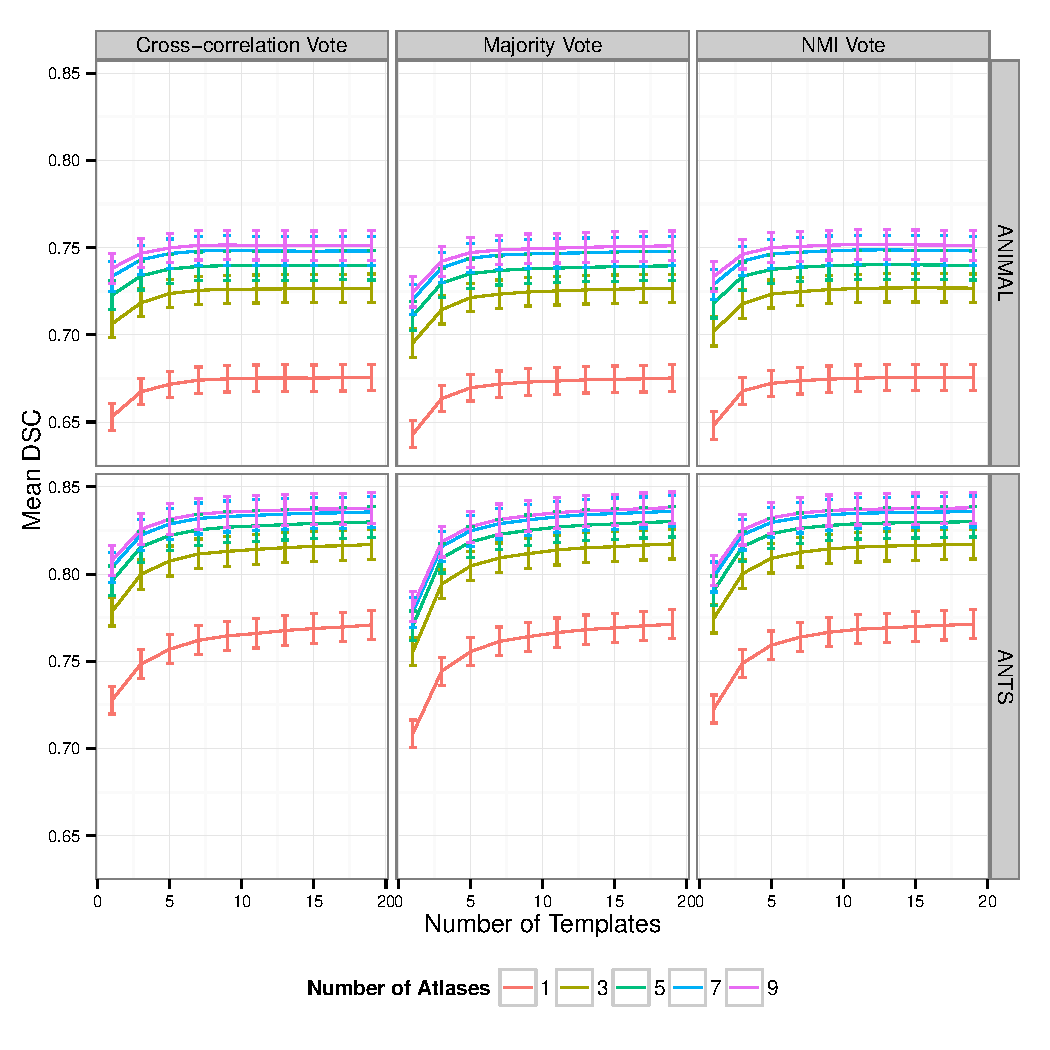
\includegraphics[width=\maxwidth]{figure/fig_ADNI1-xval-k-mean} 

}



\end{knitrout}

  \caption{Mean Dice's Similarity Coefficient of \mb segmentations with manual
  segmentations (SNT) for 69 ADNI1 subjects vs. atlas and template library size,
  registration algorithm, and label fusion method. Points above zero indicate an
  \mb parameter settings yielding a higher mean DSC score than multi-atlas
  segmentation using the same number of atlases. \label{fig:ADNI1-xval-k-mean}}
\end{figure}
%%%%%%%%%%%%%%%%%%%%%%%%%%%%%%%%%%%%%%%%

%%%%%%%%%%%%%%%%%%%%%%%%%%%%%%%%%%%%%%%%
% ADNI1-XVAL: "increase" in mean kappa over multi-atlas
\begin{figure}
\begin{knitrout}
\definecolor{shadecolor}{rgb}{0.969, 0.969, 0.969}\color{fgcolor}

{\centering 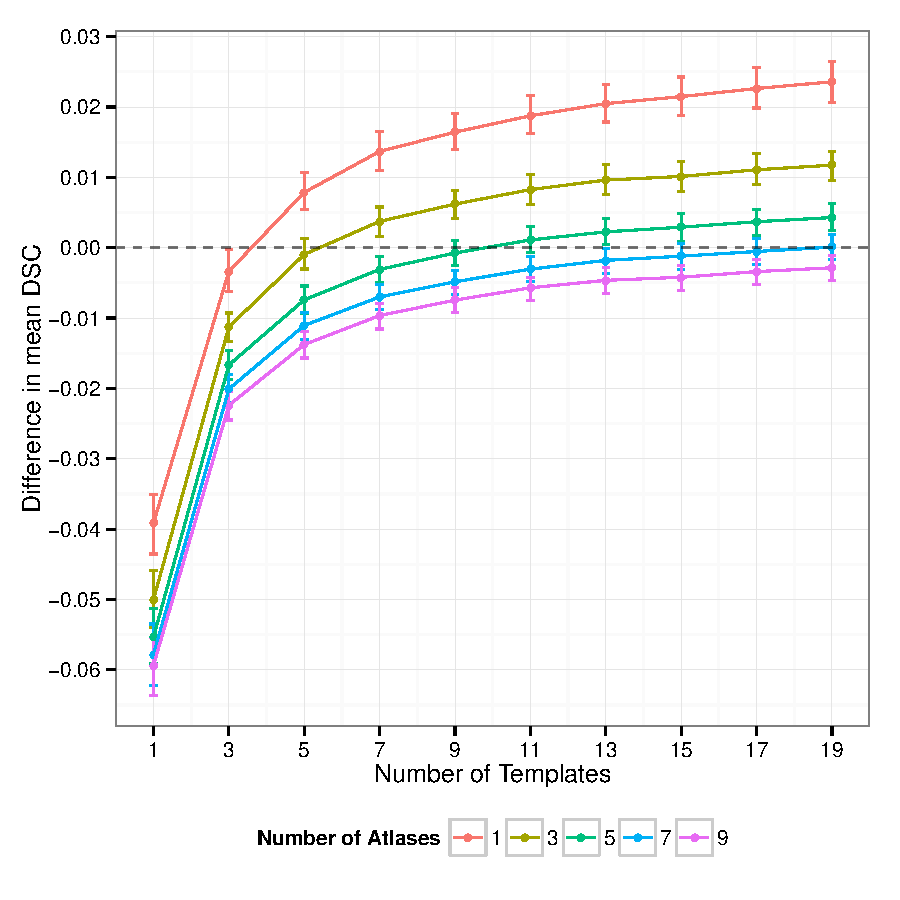
\includegraphics[width=\maxwidth]{figure/fig_ADN11-xval-k-diff} 

}



\end{knitrout}

  \caption{Difference in mean Dice's Similarity Coefficient of \mb and
  multi-atlas segmentations with manual (SNT) segmentations for a range of atlas
  and template library sizes. \label{fig:ADNI1-xval-k-diff}}
\end{figure}
%%%%%%%%%%%%%%%%%%%%%%%%%%%%%%%%%%%%%%%%

%%%%%%%%%%%%%%%%%%%%%%%%%%%%%%%%%%%%%%%%
% ADNI1-XVAL: show variability of MAGeT over parameters
\begin{figure}
\begin{knitrout}
\definecolor{shadecolor}{rgb}{0.969, 0.969, 0.969}\color{fgcolor}

{\centering 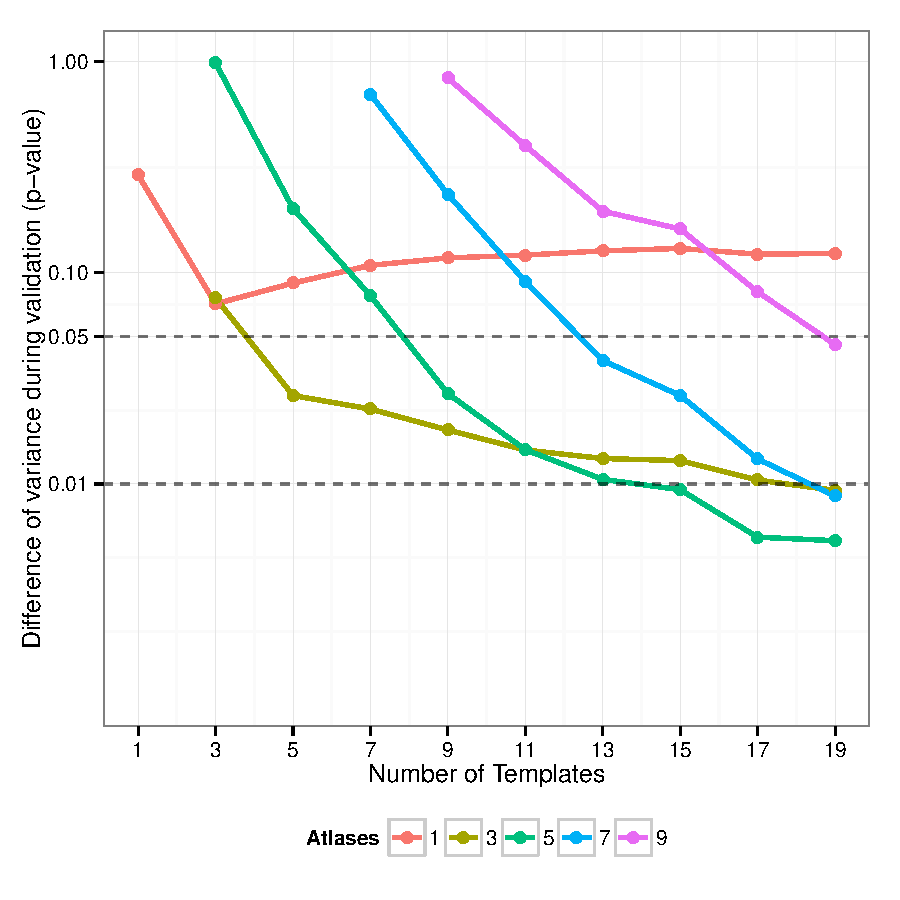
\includegraphics[width=\maxwidth]{figure/ADN1-Xval-variability} 

}



\end{knitrout}

  \caption{{\bf Difference in variability of \mb vs. multi-atlas segmentation 
  accuracy.}
  Variance of segmentation accuracy between \mb and multi-atlas segmentation 
  is computed for each subject across all ten rounds of validation. Shown on the 
  y-axis (scaled logarithmically) is the  p-value resulting from a t-test 
  comparing the distribution of variances at each parameter setting 
  (atlas/template library size). Only points where \mb mean variability is lower 
  than multi-atlas are shown.}
  \label{ADNI1-xval-variability}
\end{figure}
%%%%%%%%%%%%%%%%%%%%%%%%%%%%%%%%%%%%%%%%

\FloatBarrier

%%%%%%%%%%%%%%%%%%%%%%%%%%%%%%%%%%%%%%%%%%%%%%%%%%%%%%%%%%%%%%%%%%%%%%%%%%%%%%%
%%%%%                                                                     %%%%%
%%%%%    RESULTS: Experiment 2: Hippocampal Subfield Cross-Validation     %%%%%
%%%%%                                                                     %%%%%
%%%%%%%%%%%%%%%%%%%%%%%%%%%%%%%%%%%%%%%%%%%%%%%%%%%%%%%%%%%%%%%%%%%%%%%%%%%%%%%
\subsection{Experiment 2 Results: Winterburn Atlases Cross-Validation}
This experiment explores \mb segmentation of hippocampal subfields. To
achieve this, a leave-one-out validation is conducted in which lower-resolution
images ($0.9mm^3$ voxels) of each Winterburn atlas subject are segmented using 
the remaining Winterburn atlases. 

In general, across hippocampal subregions the percent error in volume of
\mb segmentations compares
favourably to the error resulting from image resampling (Figure
\ref{fig:WAval-vol-boxplot}). In particular, the CA1, CA4, and Dentate
subregions all show near or smaller percent errors. The Sibiculum and CA2/CA3
subregions show distinctly larger error than is found through resampling.  

Figure \ref{fig:subfield-montage} shows a qualitative comparison of \mb subfield
segmentation.  


%%%%%%%%%%%%%%%%%%%%%%%%%%%%%%%%%%%%%%%%
% Winterburn-XVAL: compare resampling
\begin{figure}[h!]
\begin{knitrout}
\definecolor{shadecolor}{rgb}{0.969, 0.969, 0.969}\color{fgcolor}

{\centering 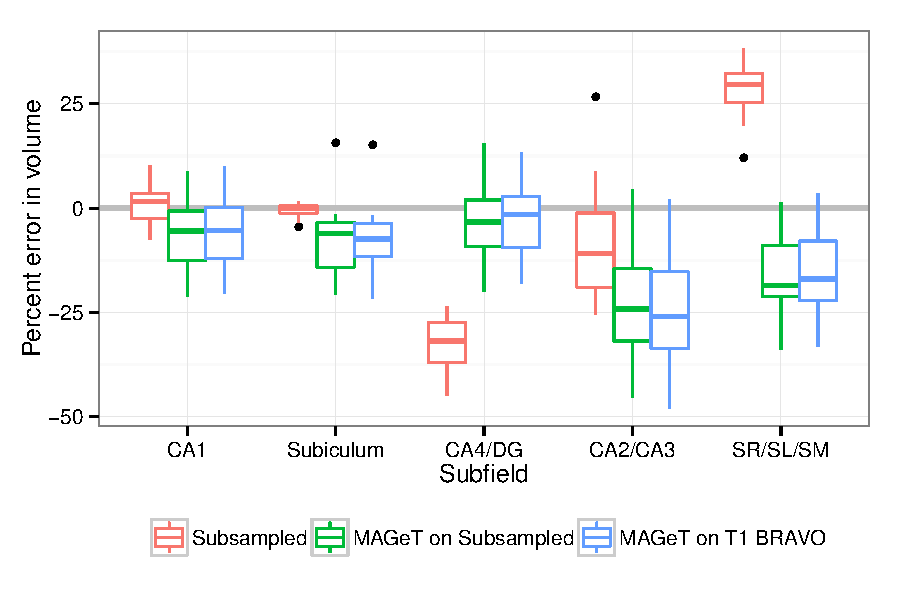
\includegraphics[width=\maxwidth]{figure/WAval-vol-boxplot} 

}



\end{knitrout}

  \caption{{\bf Percent error in segmentation volume by hippocampus subregion.} 
  Percent error is measured against the volumes of of the unmodified Winterburn
  atlas segmentations.
  {\bf Subsampled} are volumes of the manual segmentations of the Winterburn
  atlases after resampling to $0.9mm^3$.  
  {\bf MAGeT + WA Subsampled} volumes are \mb segmentations of the Winterburn atlas
  images after resampling to $0.9mm^3$ voxels.
  {\bf MAGeT + WA BRAVO} volumes are \mb segmentations of T1 BRAVO images
  ($0.9mm^3$ voxels) acquired separately of four of the five Winterburn atlas
  subjects.} 
  \label{fig:WAval-vol-boxplot}
\end{figure}


\begin{figure}
  \begin{centering}
    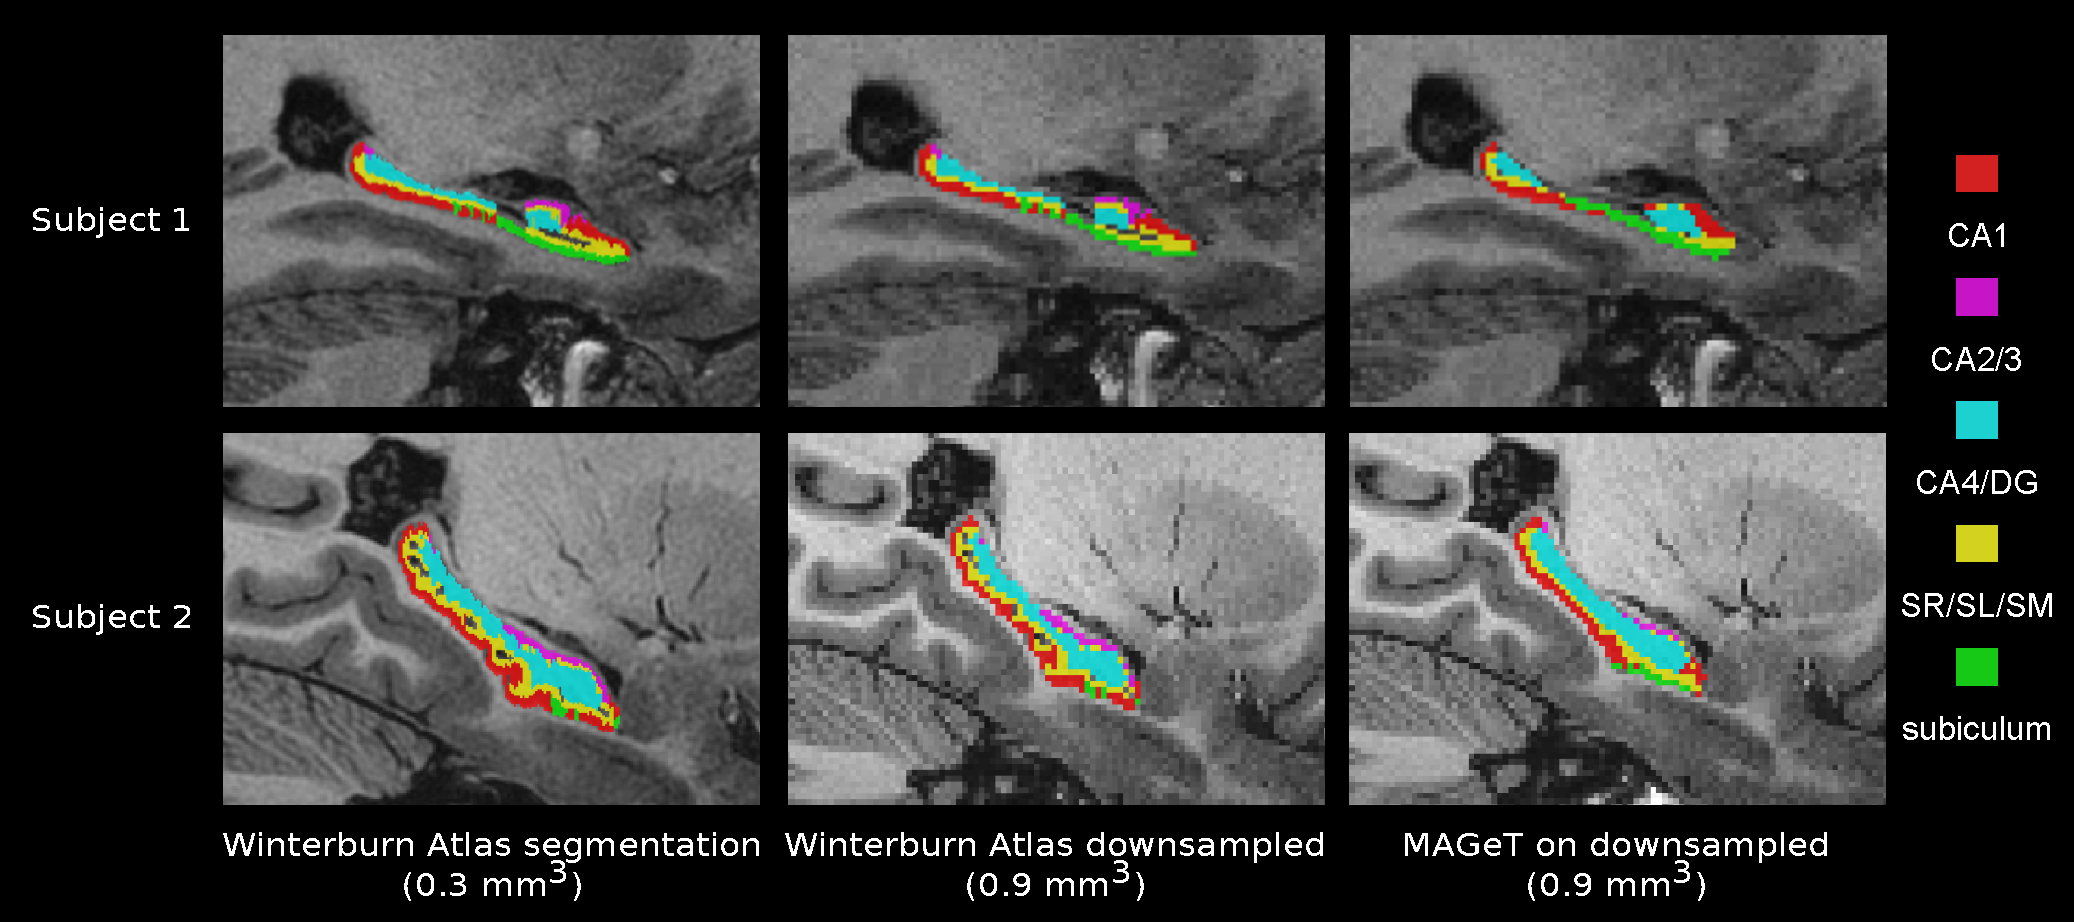
\includegraphics[width=6in]{figure/subfield-montage.pdf}
  \end{centering}
  \caption{Sagittal slices from two subjects showing a comparison of the
  original Winterburn atlas subfield segmentations (at 0.3mm-isotropic voxel
  resolution), the subsampled Winterburn segmentations (at 0.9mm-isotropic
  voxel resolution), and the \mb labels on the subsampled atlas image.}
  \label{fig:subfield-montage}
\end{figure}

\todo[inline]{Figure \ref{fig:subfield-montage}. Show MAGeT segmentations on
BRAVO images.  Also, show coronal/transverse slices and MNI coordinates}

\FloatBarrier
%%%%%%%%%%%%%%%%%%%%%%%%%%%%%%%%%%%%%%%%%%%%%%%%%%%%%%%%%%%%%%%%%%%%%%%%%%%%%%%
%%%%%                                                                     %%%%%
%%%%%    RESULTS: Experiment 3, Application of \mb to the segmentation    %%%%%
%%%%%                       of schizophrenia patients                     %%%%%
%%%%%                                                                     %%%%%
%%%%%%%%%%%%%%%%%%%%%%%%%%%%%%%%%%%%%%%%%%%%%%%%%%%%%%%%%%%%%%%%%%%%%%%%%%%%%%%
\subsection{Experiment 3 Results: Application to the segmentation of first episode
\\ \mbox{schizophrenia patients}}
 
In this experiment \mb is applied to a dataset of images of first episode
schizophrenia patients, using the Winterburn atlases and a template library of
21 subject images selected at random.  Expert manual whole hippocampal
segmentations are used as gold standards. 

\begin{figure}
\begin{knitrout}
\definecolor{shadecolor}{rgb}{0.969, 0.969, 0.969}\color{fgcolor}

{\centering 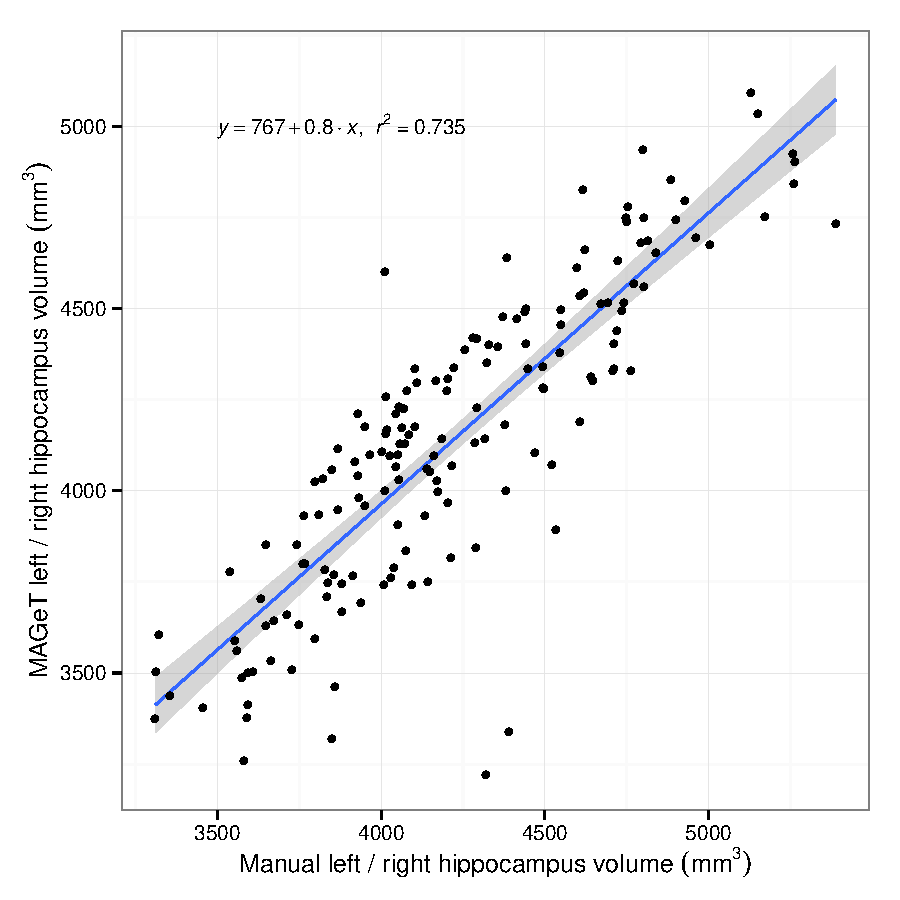
\includegraphics[width=\maxwidth]{figure/FEP-volumes} 

}



\end{knitrout}

  \caption{Subject mean hippocampal volumes by \mb vs. manually segmented
   volumes from the First Episode Patients with Schizophrenia dataset. A linear fit
   and standard error are shown.}
  \label{fig:SZ-volumes}
\end{figure}



\mb produces hippocampus segmentation volumes that are highly correlated with 
manual segmentation volumes (Pearson $r = 0.877$, 
$t = 16.244$, $p < 0.001$; Figure \ref{fig:SZ-volumes}). 


\FloatBarrier
%%%%%%%%%%%%%%%%%%%%%%%%%%%%%%%%%%%%%%%%%%%%%%%%%%%%%%%%%%%%%%%%%%%%%%%%%%%%%%%
%%%%%                                                                     %%%%%
%%%%%                           RESULTS                                   %%%%%
%%%%%                                                                     %%%%%
%%%%%         EXPERIMENT 4: Application of \mb to the segmentation        %%%%%
%%%%%                       of ADNI subjects                              %%%%%
%%%%%                                                                     %%%%%
%%%%%%%%%%%%%%%%%%%%%%%%%%%%%%%%%%%%%%%%%%%%%%%%%%%%%%%%%%%%%%%%%%%%%%%%%%%%%%%
\subsection{Experiment 4 Results: Application to the segmentation of Alzheimer's
disease patients}

Based on the results from the ADNI1 Cross-Validation experiment, in this
experiment \mb was configured with a template library of 21 randomly chosen
subject images (7 from each disease class) and used majority vote label fusion.
The entire \adnidataset dataset was segmented by \mb and we now compare the
resulting volumes with those obtained by manual segmentation (SNT), and other
automated segmentation techniques (MAPER, FreeSurfer, and FSL).  Table
\ref{tab:ADNI1-1.5T-Complete-1Yr-Dataset-Method-Totals} shows the total count of
segmentations available, including a count of those which have failed a quality
control inspection. Quality control for FreeSurfer segmentations was provided along
with the segmentations from ADNI \cite{Hartig2010}. One of the authors (MP) 
performed visual quality inspection for MAGeT and FSL segmentations using similar 
quality control guidelines (if either hippocampus was under or over segmented
by greater than 10mm in three or more slices then the segmentation did not pass). 

Only those images which had quality segmentations from each method are 
included in the following analysis (a total of 361
images).
 
We find a close relationship in total bilateral hippocampal volume between
all methods and manually segmented volumes (Figure \ref{fig:ADNI-volumes-plot}). 
Volumes are correlated with Pearson $r > 0.78$ for all methods across disease
categories.  Within disease categories (Figure \ref{fig:ADNI-volumes-boxplot}),
\mb is consistently well correlated to manual volumes (Pearson $r > 0.85$), but
appears to slightly over-estimate the volume of the AD hippocampus. 

To investigate the level of agreement with manually segmented hippocampal
volumes, we constructed Bland-Altman plots for each method (Figure
\ref{fig:ADNI-Bland-Altman}).  As \citet{Bland1986} noted, high correlation
amongst measures of the same quantity does not necessarily imply agreement (as
correlation can be driven by a large range in true values, for instance).  What
is most striking in Figure \ref{fig:ADNI-Bland-Altman} is that all methods show
an obvious proportional bias: FreeSurfer and FSL markedly under-estimate smaller
hippocampi and over-estimate large hippocampi, whereas MAPER and \mb more
conservatively show the reverse bias.  Additionally, all methods show a fixed
bias, with FreeSurfer and FSL most dramatically over-estimating hippocampal
volume by $2600 mm^3$ and $2800 mm^3$ on average, respectively, and MAPER and
\mb within $250 mm^3$ on average. 

Figure \ref{fig:ADNI-subfields} shows a qualitative comparison of \mb and 
manual (SNT) hippocampal segmentations for 10 randomly selected subjects in 
each disease category, and illustrates some of the common errors found during 
visual inspection. Mostly frequently, we find \mb improperly includes the vestigial
hippocampal sulcus and, although not anatomically incorrect, \mb under-estimates 
the hippocampal body in comparison to the manual (SNT) segmentation.  

%%%%%%%%%%%%%%%%%%%%%%%%%%%%%%%%%%%%%%%%
% ADNI1 1yr Complete Dataset Package Totals & Failures
%                        
% latex.default(package_totals, file = "", size = "scriptsize",      landscape = FALSE, ctable = TRUE, caption = "\\textbf{Number of segmented images and quality control failures of \n             \\adnidataset dataset by method.}",      caption.loc = c("top"), rowname = NULL, label = "tab:ADNI1-1.5T-Complete-1Yr-Dataset-Method-Totals") 
%
{\scriptsize\ctable[caption={\textbf{Number of segmented images and quality control failures of 
             \adnidataset dataset by method.}},label=tab:ADNI1-1.5T-Complete-1Yr-Dataset-Method-Totals,pos=!tbp,]{llrlrr}{}{\FL
\multicolumn{1}{c}{X}&\multicolumn{1}{c}{SNT}&\multicolumn{1}{c}{MAGeT}&\multicolumn{1}{c}{MAPER}&\multicolumn{1}{c}{FSL}&\multicolumn{1}{c}{FS}\ML
Images&1445&$1909$&636&$1876$&$1530$\NN
Failures&--&$  34$&--&$  27$&$ 304$\LL
}}


%%%%%%%%%%%%%%%%%%%%%%%%%%%%%%%%%%%%%%%%


\begin{figure}[h]
\begin{knitrout}
\definecolor{shadecolor}{rgb}{0.969, 0.969, 0.969}\color{fgcolor}

{\centering 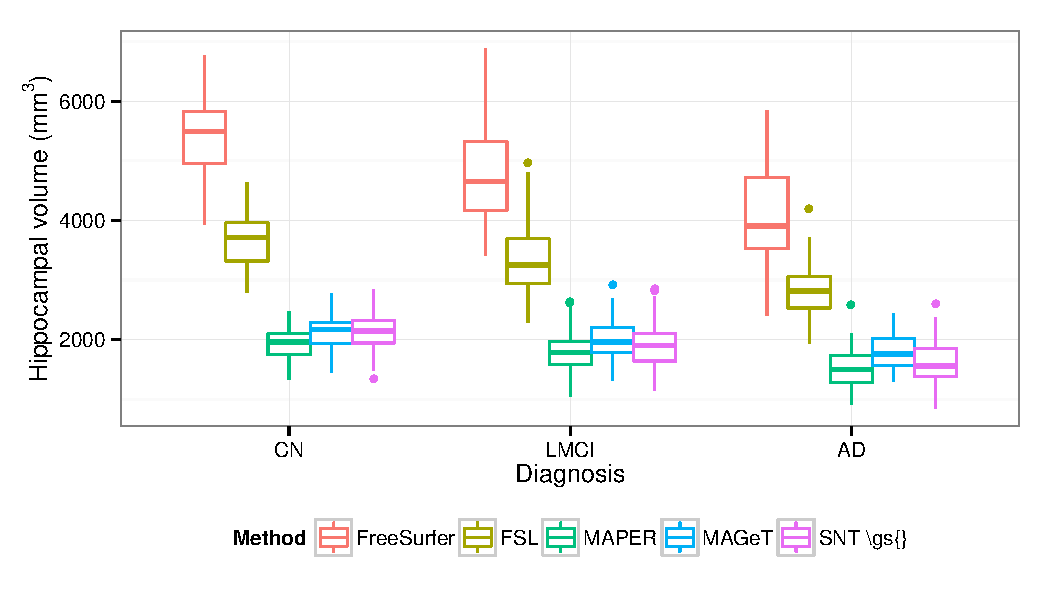
\includegraphics[width=\maxwidth]{figure/ADNI-volumes-boxplot} 

}



\end{knitrout}

  \caption{Subject mean hippocampal volume as measured in the \adnidataset
dataset by FreeSurfer, FSL, MAPER, \mb, and manual raters (SNT) vs. disease
category.}
  \label{fig:ADNI-volumes-boxplot}
\end{figure}

\begin{figure}[h]
\begin{knitrout}
\definecolor{shadecolor}{rgb}{0.969, 0.969, 0.969}\color{fgcolor}

{\centering 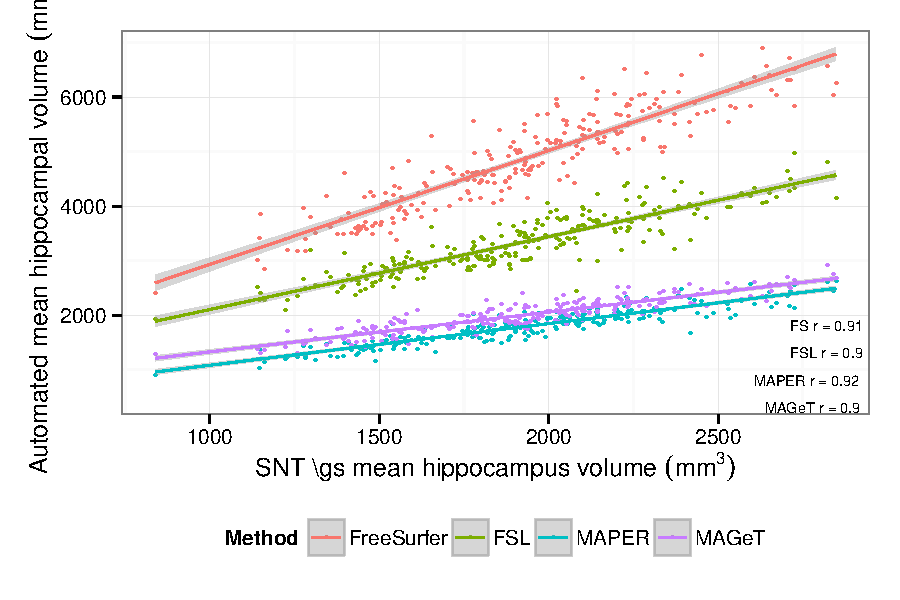
\includegraphics[width=\maxwidth]{figure/ADNI-volumes-plot} 

}



\end{knitrout}

  \caption{Subject mean hippocampal volume as measured in the \adnidataset
dataset by each of the four automated methods investigated (FreeSurfer (FS),
FSL, MAPER, \mb) vs. manual rating (SNT). Linear fit lines and pearson
correlations are shown for each method.}
  \label{fig:ADNI-volumes-plot}
\end{figure}
 
\begin{figure}
\begin{knitrout}
\definecolor{shadecolor}{rgb}{0.969, 0.969, 0.969}\color{fgcolor}

{\centering 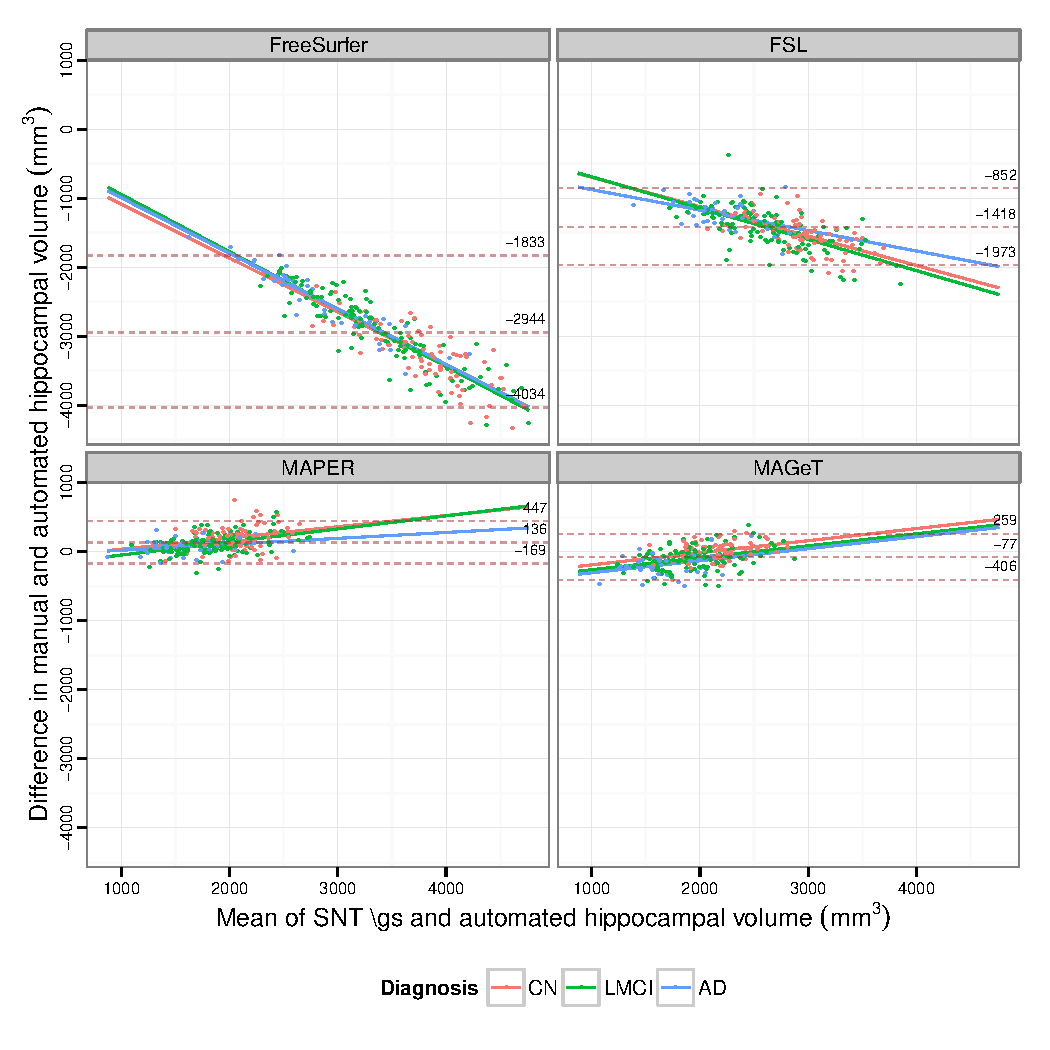
\includegraphics[width=\maxwidth]{figure/ADNI-Bland-Altman} 

}



\end{knitrout}

  \caption{Bland-Altman plots comparing subject mean hippocampal volume as
measured in the \adnidataset dataset by manual raters (SNT) and each of the four
automated methods investigated (FreeSurfer, FSL, MAPER, \mb). The overall mean
difference in volume, and limits of agreement ($\pm 1.96SD$) are shown by dashed
horizontal lines. Linear fit lines are shown for each diagnosis group. Note,
points below the mean difference indicate overestimation of the volume with
respect to the manual rating, and vice versa. }

  \label{fig:ADNI-Bland-Altman}
\end{figure}




\begin{figure}
  \begin{centering}
    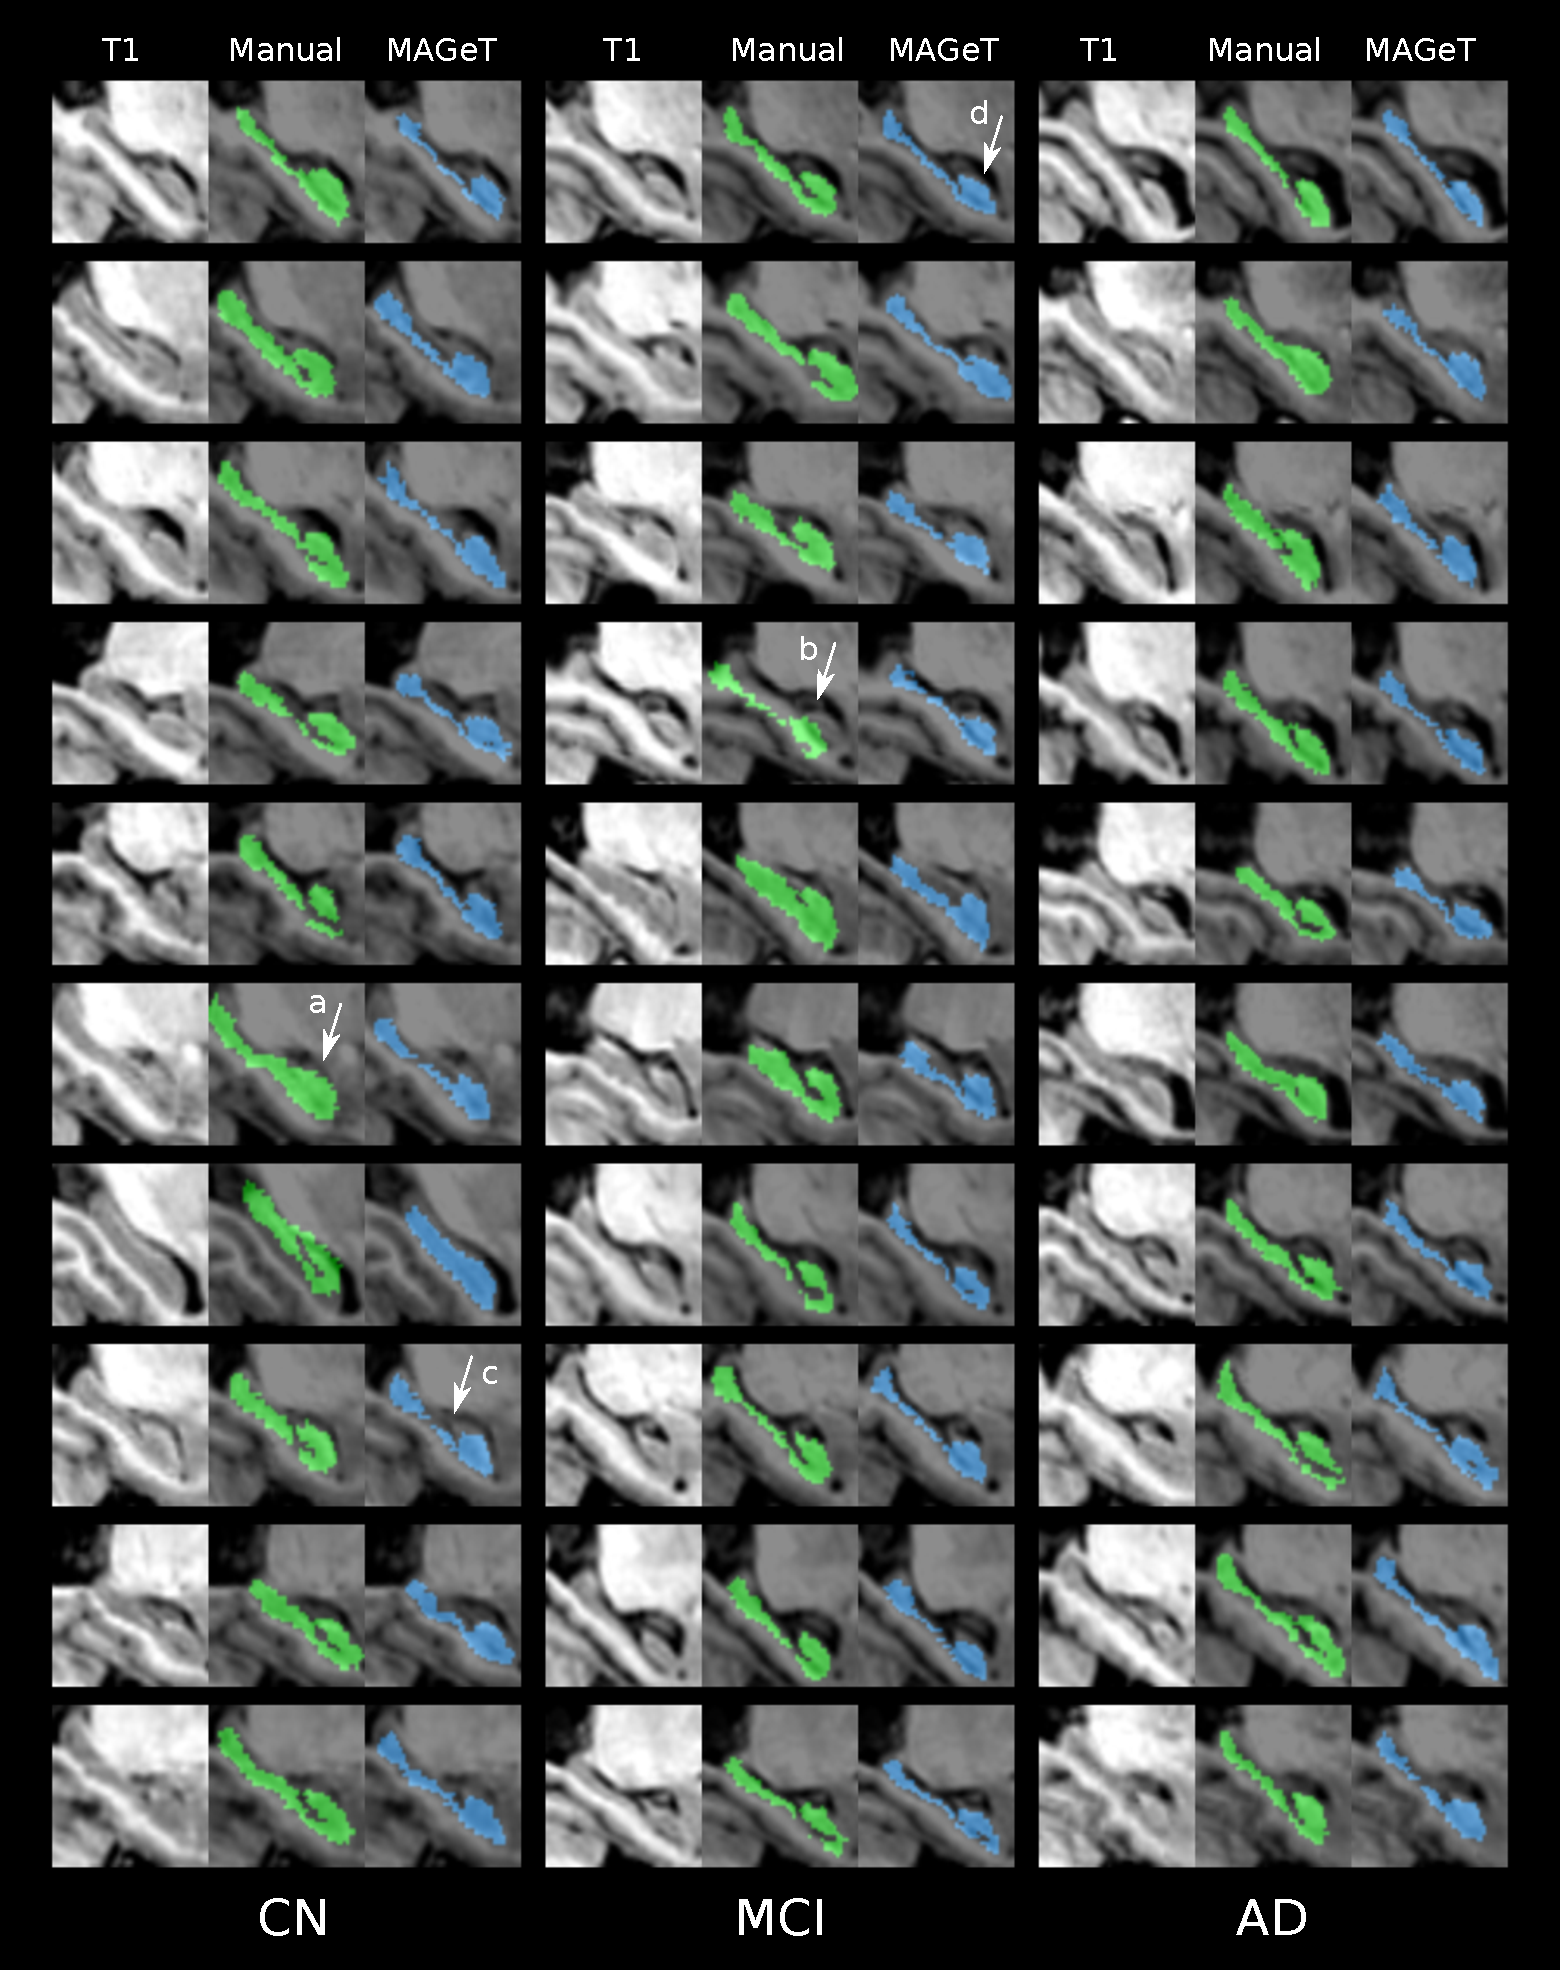
\includegraphics[width=6in]{figure/ADNI1_SNT_MB_montage/montage.pdf}
  \end{centering}
  \caption{Manual and MAGeT segmentation results for 30 ADNI1 subjects (10
  subjects randomly selected from each disease category in the subject pool used
  in Experiment 1). Sagittal slices are shown for subject unlabelled T1-weighted
  anatomical image, SNT manual label (green), and \mb label (blue). Noted are
  examples of common segmentation idiosyncrasies: 
  {\em (a)} over-estimation of hippocampal head and  
  {\em (b)} translated manual segmentation by SNT; 
  {\em (c)} under-estimation of hippocampal body and
  {\em (d)} improper inclusion of the vestigial hippocampal sulcus by \mb.}
  \label{fig:ADNI-subfields}
\end{figure}

\todo[inline]{Figure \ref{fig:ADNI-subfields}. Show coronal/transverse slices
and MNI coordinates}

\FloatBarrier

%%%%%%%%%%%%%%%%%%%%%%%%%%%%%%%%%%%%%%%%%%%%%%%%%%%%%%%%%%%%%%%%%%%%%%%%%%%%%%%%
%                                Discussion
%%%%%%%%%%%%%%%%%%%%%%%%%%%%%%%%%%%%%%%%%%%%%%%%%%%%%%%%%%%%%%%%%%%%%%%%%%%%%%%%
\section{Discussion}
%%%%%%%%%%%%%%%%%%%%%%%%%%%%%%%%%%%%%%%%
% Tabulation of segmentation accuracies of existing methods (ADNI)
%


%%%%%%%%%%%%%%%%%%%%%%%%%%%%%%%%%%%%%%%%

%%%%%%%%%%%%%%%%%%%%%%%%%%%%%%%%%%%%%%%%
% Tabulation of segmentation accuracies of existing methods (ADNI)
%
%



\begin{table*}[!tbp]
\scriptsize
\caption{\textbf{Automated segmentation accuracy (overlap with manual labels) of the 
   ADNI dataset.} For each method, the number of manually labelled atlases used for 
   training, the best Dice's overlap measure, the disease classes measured, and 
   the validation procedure are shown. Unless specified, validation datasets are
   composed equally of subjects diagnosed with Alzheimer's Disease (AD), Mild 
   Cognitive Impairment (MCI), and Cognitively Normal (CN). LOOCV = Leave-one-out 
   cross-validation. 
   Some studies of automated segmentation of ADNI images are excluded because they 
   do not not provide overlap measures for the hippocampus \cite{Heckemann2011,Chupin2009}.
  \label{tab:other-methods}} 
\begin{center}
\begin{tabular}{ l  c  p{1in}  l  p{2in}  }
\hline\hline
Method & Atlases & DSC & Reference & Validation \tabularnewline
\hline
\mb                     &9 & 0.838 & & 10 rounds of Monte Carlo CV on a pool of 69 subjects \tabularnewline
LEAP                    &30&0.848                 &\cite{Wolz2010}  &Segmentation of 60 subjects\tabularnewline
ACM (AdaBoost-based)    &21&0.862                 &\cite{Morra2008} &LOOCV on atlases\tabularnewline
Patch-based label fusion&16&0.883 (CN) \newline 0.838 (AD)&\cite{Coupe2011e}&LOOCV on atlases\tabularnewline
Multi-atlas             &30&0.885                 &\cite{Lotjonen2010}&Segmentation of 60 subjects\tabularnewline
Multi-atlas + weighted fusion&20&0.898 (CN) \newline 0.798 (left HC, MCI) &\cite{Wang2011}  &10 rounds of Monte Carlo CV on 20 subjects, pool of 139 (CN/MCI)\tabularnewline
Multi-atlas (MAPS)    &55&0.890                   &\cite{Leung2010}&Segmentation of 30 subjects (10 AD, MCI, and CN)\tabularnewline
\hline
\end{tabular}
\end{center}
\end{table*}

In this manuscript we have presented the implementation and validation of the
\mb framework -- a methodology that requires very few input atlases in
order to provide accurate and reliable segmentations.  We have demonstrated that
our methodology robustly provides accurate and consistent segmentations in
populations with different ageing and neuropsychiatric characteristics.
Further, we have demonstrated that algorithmic performance is not dependent on a
single definition of the hippocampus but is effective with differing hippocampal
definitions \citep{Winterburn2013,Pruessner2000,Hsu2002}.  Finally, we also demonstrate
that \mb provides accurate automatic identification of the hippocampal
subfields despite contrast and resolution limitations in standard T1-weighted
image volumes. 

Throughout the cross validation in Experiment 1 (10-fold Monte Carlo cross 
validation in the
\adnidataset dataset subsample) we find that two parameter choices improve 
segmentation accuracy: increasing the number of atlases, and the number of
templates. However, after setting the parameters to 5 atlases and 15 templates
there are diminishing returns with respect to this improvement. We were
somewhat surprised to find that cross-correlation and normalized mutual
information based weighted voting did little to improve segmentation accuracy.
This suggests that using an intermediate template library generated by accurate
nonlinear registration methods such as \ants \citep{Avants2008} sufficiently filters
sources of error such as nonlinear registration error and partial volume effects
that arise through the use of nearest neighbour resampling. From our previous
work on the \mb algorithm we have shown that these increases in error
are not simply a smoothing or averaging effect \citep{MallarChakravarty2012}.

Although, the goal of this manuscript was to not exhaustively test or validate
multiple different voting strategies in the context of our segmentation
algorithm, it is important to note that other strategies for voting are
available.  For example, other groups have used the STAPLE algorithm
\citep{Warfield2004} (or variants of the STAPLE algorithm \citep{Robitaille2012})
which weights each segmentation based upon its estimated
performance level with respect to the other available candidate segmentations.
Further, the sensitivity and specificity parameters could also be tuned to
potentially improve segmentation accuracy and reliability.  It is rather likely
that using more sophisticated voting methods would have a positive effect on the
overall segmentation performance.  

To this end, more work is required in order to determine the source of the
slight decrease in segmentation performance when the number of templates are set
to an even number.  Our initial concern was that this dip in performance was a
by-product of the \mb algorithm itself.  However, we determined that
this pattern was also true in the analysis of multi-atlas segmentations we used
in our experiments.  We believe that our majority voting methodology is biased
towards labels with the lowest numeric values when breaking ties, thus causing
the slight bias observed when using an even number of templates. This is another
area where the voting scheme could be used to improve performance. However, it
is worth noting that this limitation was previously identified by
\citet{Heckemann2006a} and, subsequently, other groups have not even considered
the potential pitfalls of an even number of candidate labels (eg.
\citet{Leung2010}).

Another concern is the moderate-to-small improvement observed in \mb in
comparison to multi-atlas segmentation when using the same number of atlases.
The actual benefit in using \mb is consistency of the labelling regardless of
atlas or template choice. This is an important consideration that few have
touched on previously. The 10-fold Monte Carlo leave-one-out cross-validation that we present
in Experiment 1 is amongst one of the most stringent performed in the
multi-atlas/segmentation literature.  To the best of our knowledge, other groups
using ADNI data for validation do at most a single round of leave-one-out-validation
(Table \ref{tab:other-methods}), aside from \citep{Wang2011} who perform a 
similar validation as us. The thoroughness of our validation suggests that
our results are reflective of a true average over the choice of parameter
settings and are independent of atlas or template choice (provided the input
atlases are properly segmented).  

% Validation of ADNI in other works
% Chupin 2009: LOOCV, 1-fold validation
% Heckemann 2011: QC of segmentations, comparison across field strengths, 
%                 agreement between two different atlas sets
% Coupe 2011e: LOOCV
% Lotjonen 2010: LOOCV, 1-fold validation
% Leung 2010: 1-fold, QC, classification
% Wolz 2010: 1-fold over different leap settings, classification
% Collins 2010: 1-fold validation, QC
% Morra 2008: LOOCV with 21 atlases, 2 manual raters
% Wang 2011: 10 rounds of MCCV with 20 atlases and 20 subjects, chosen from 
%            a pool of 139 images


\todo[inline]{could we be seeing a ceiling effect... reaching the limit of what
is achievable with a multi-atlas-based segmentation method}

In comparison to other methodologies in the field, it is important to note that
\mb performs quite well.  Table 6 gives a survey of some of the most recent
multi-atlas implementations with the reported kappa values used to validate the
algorithm on the ADNI dataset (many of which use the same SNT labels for
populating their template library and as gold standards for evaluation).  While
it is difficult to compare segmentation results across studies, gold-standards,
evaluation metrics, and algorithms it is worth noting that the methods
summarized in Table 6 require more atlases (between 16-55) than our \mb
implementation with the Winterburn atlases \citep{Winterburn2013}.  Amongst these
methods only method 4 yields mean Kappas that are higher than the ones that are
reported here.  

There are some important differences between our method
and these specific methods.  Others have reported the difficulty with
mis-registrations in candidate segmentation (i.e. segmentations generated that are
then input in the voxel-voting procedure \citep{Collins2010}). The work of 
\citet{Leung2010} tackles this problem by using an intensity threshold
that is estimated heuristically at the time of segmentation (this work also
reports some of the highest kappas for the segmentation of ADNI data).  While
this works for the ADNI dataset (which is partially homogenized with respect to
image acquisition and pre-processing), it is unclear if this type of heuristic
is applicable to other datasets.  In all cases, these methods require more
atlases than our implementation with the Winterburn atlases.
\citet{Lotjonen2010} achieve highly accurate segmentation but correct their
segmentations using classifications derived using an expectation maximization
framework.  In their initial work, \citet{Chupin2009} develop their
probabilistic methodology using a cohort of 8 healthy controls and 15 epilepsy
patients.  In subsequent methods, they retuned their methodology using the ADNI
sample with a hierarchical experimentation protocol that involved.  These
methods suggest that some post-processing of the final segmentations would
improve accuracy of the segmentation.  While that may be true, there is little
consensus regarding how to achieve this.  

To the best of our knowledge, no other groups have validated their work using
multiple atlas segmentation protocols, different acquisitions, and disease
populations in order to demonstrate the robustness of their technique.  This is
one of the clear strengths of this work.  Furthermore, unlike some of the
algorithms mentioned, our implementation does not require retuning for new
populations or datasets as it inherently models the variability of the dataset
through the template library.  However it should be noted that the increased
accuracy that follows increasing the number of atlases and templates comes at an
increased computational cost ($O(log(n))$), as previously mentioned in
other work \citep{Heckemann2006}. 
\todo[inline]{time complexity seems suspicious} 

In comparison to the methods that we compared and were available through the
ADNI database (FreeSurfer, MAPER) and the method that we initialized ourselves
(FSL-FIRST) we find extremely variable performance of all methods.  With the
exception of FSL all methods correlate well with the SNT volumes provided in
the ADNI database.  However, FreeSurfer and FIRST provide radically different
definitions of the size of the hippocampus in comparison to the other methods.
Further, when estimating bias of these methods relative to SNT hippocampal
volumes we see that large hippocampi are over estimated while small hippocampi
are under estimated.  By comparison, our method and MAPER are far more
conservative suggesting that these methods may be better suited for estimating
true-positives.  While this comparison with these methods using only volume,
more work is needed to better understand the differences between our method and
other methods.

Finally, we have also demonstrated that our algorithmic framework is appropriate
for the segmentation of hippocampal subfields in standard T1-weighted data.
This has started to become a burgeoning topic in the segmentation literature,
although very few methods are available for the segmentation of 3T data
\citep{Yushkevich2009,VanLeemput2009}. However, the FreeSurfer implementation of
subfield segmentation. While recent work demonstrates that subfield
segmentations can be used for classification of AD, MCI, and NC, there has been
no explicit validation of the methodology based on accuracy or precision.
Although the initial hippocampal subfield segmentations from the Yushkevich
group have been demonstrated to work on the ADNI population, there has also been
no validation of their work.  In addition, their work requires some manual
initialization to properly function.  Our work demonstrates that we can reliably
identify the CA1, subiculum, and CA4 dentate with only modest amounts of error.
The fact that CA2/CA3 and molecular layers cannot be reasonably identified
should not be surprising.  These are extremely thin and spatially convoluted
regions that originally required high-resolution MRI for identification.  It is
likely that they would be that extents of these regions are well below the
resolution offered by standard T1-weighted images.  In fact many manual
segmentation methodologies do not attempt to parse these regions either
\citep{Wisse2012, Mueller2009}

\subsection{Conclusion}
In conclusion, we have presented a flexible multi-atlas framework.  It has
considerable advantages over other methods as only a small set of atlases is
required to initialize the algorithm.  We demonstrate that our method works
robustly over hippocampal definitions, different populations, and different
acquisition types.  Finally, we also demonstrate that using this method that
accurate identification of the hippocampal subfields in also possible.

%%%%%%%%%%%%%%%%%%%%%%%%%%%%%%%%%%%%%%%%%%%%%%%%%%%%%%%%%%%%%%%%%%%%%%%%%%%%%%%%
%                               Conclusion 
%%%%%%%%%%%%%%%%%%%%%%%%%%%%%%%%%%%%%%%%%%%%%%%%%%%%%%%%%%%%%%%%%%%%%%%%%%%%%%%%

\section{Supplementary Materials}

\subsection{ADNI Manual Labels}
% The following blurb is taken (except for the first sentence) verbatim 
Semi-automated hippocampal volumetry was carried out using a commercially
available high dimensional brain mapping tool (Medtronic Surgical Navigation
Technologies, Louisville, CO), that has previously been validated and compared
to manual tracing of the hippocampus \citep{Hsu2002}. Measurement of hippocampal
volume is achieved first by placing manually 22 control points as local
landmarks for the hippocampus on the individual brain MRI data: one landmark at
the hippocampal head, one at the tail, and four per image (i.e., at the
superior, inferior, medial and lateral boundaries) on five equally spaced images
perpendicular to the long axis of the hippocampus. Second, fluid image
transformation is used to match the individual brains to a template brain
\citep{Christensen1997}. The pixels corresponding to the hippocampus are then
labeled and counted to obtain volumes. This method of hippocampal voluming has a
documented reliability of an intraclass coefficient better than .94
\citep{Hsu2002}.

\bibliographystyle{abbrvnat}
\bibliography{references}
\end{document}
